\documentclass{report}
\usepackage[utf8]{inputenc}
\usepackage[T1]{fontenc}
\usepackage[frenchb]{babel}
\usepackage{amssymb}
\usepackage{mathtools}
\usepackage{listingsutf8}
\usepackage{verbatim}
\usepackage{xcolor}
\usepackage{graphicx}
\usepackage[toc,page]{appendix}

\lstloadlanguages{R}

\begin{document}
\lstset{
    language=R,
    basicstyle=\footnotesize,
    numbers=left,
    backgroundcolor=\color{white},
    breakatwhitespace=false,
    breaklines=true,
    captionpos=b,
    commentstyle=\color{green},
    extendedchars=true,
    keepspaces=true,
    keywordstyle=\bfseries\color{blue},
    numbersep=5pt,
    numberstyle=\tiny\color{gray},
    showtabs=false,
    stringstyle=\color{red},
    tabsize=2,
    title=\lstname
}

\title{SY09 - TP2}
\date{Avril 2016}
\author{Stéphane LOUIS et Paul GOUJON}
\pagenumbering{gobble}
\maketitle

\newpage
\tableofcontents{}

\newpage
\pagenumbering{arabic}
\chapter{TP2 - Classification automatique}
\section{Introduction}
Ce document présente les résultats obtenus par notre binôme au cours de ce second TP de SY09.
\section{Code : Annexes}
Vous trouverez au sein des fichiers \verb+.R+ fournis en annexes les principales instructions \verb+R+ utilisées au cours de ce TP.
\section{Classification automatique non supervisée}
La classification automatique, comme toutes les méthodes de data mining, a pour but d'obtenir une représentation simplifiée de données initiales. La classification est l'organisation d'un ensemble en classes homogènes, ou classes naturelles. La classification automatique, encore appelée clustering, ou taxonomie numérique, recouvre l'ensemble des méthodes permettant la construction automatique de telles classifications.
\section{Objectif}
L'objectif général de ce TP est de mettre en pratique les connaissance en classification automatique vues en cours. Pour cela nous allons travailler sur trois datasets standards (Iris, Crabs et Mutations), auxquels nous allons appliquer différents méthodes de data mining, notamment dans un premier temps l'Analyse en Composantes Principales (ACP) et l'Analyse Factorielle de Tableau de Distances afin d'obtenir une première visualisation des données, puis dans un second temps différentes méthodes de classification automatique, notamment les classifications hiérarchique ascendantes et descendantes ainsi que la méthode des centres mobiles (méthode des k-means).

\newpage
\chapter{Exercice 1 - Visualisation des données}
\paragraph{Introduction}
L'objet de ce premier exercice est de visualiser les données qui seront étudiées dans la suite du TP.
\section{Analyse descriptive du jeu de données Iris}
\paragraph{Introduction}
Le jeu de données Iris de Ficher ou Anderson est un jeu de données standard de R donnant les mesures en centimètres des variables "sepal length and width and petal length and width" des espèces Setosa, Versicolor et Virginica d'Iris. Nous étudions tout d'abord les caractéristiques générales du jeu de données.
\paragraph{Représentation dans le premier plan factoriel - Pas de différenciation en fonction de l'espèce}
Dans un premier temps, utilisons l'ACP afin d'afficher les données dans le premier plan factoriel.
\begin{figure}[ht!]
\begin{center}
    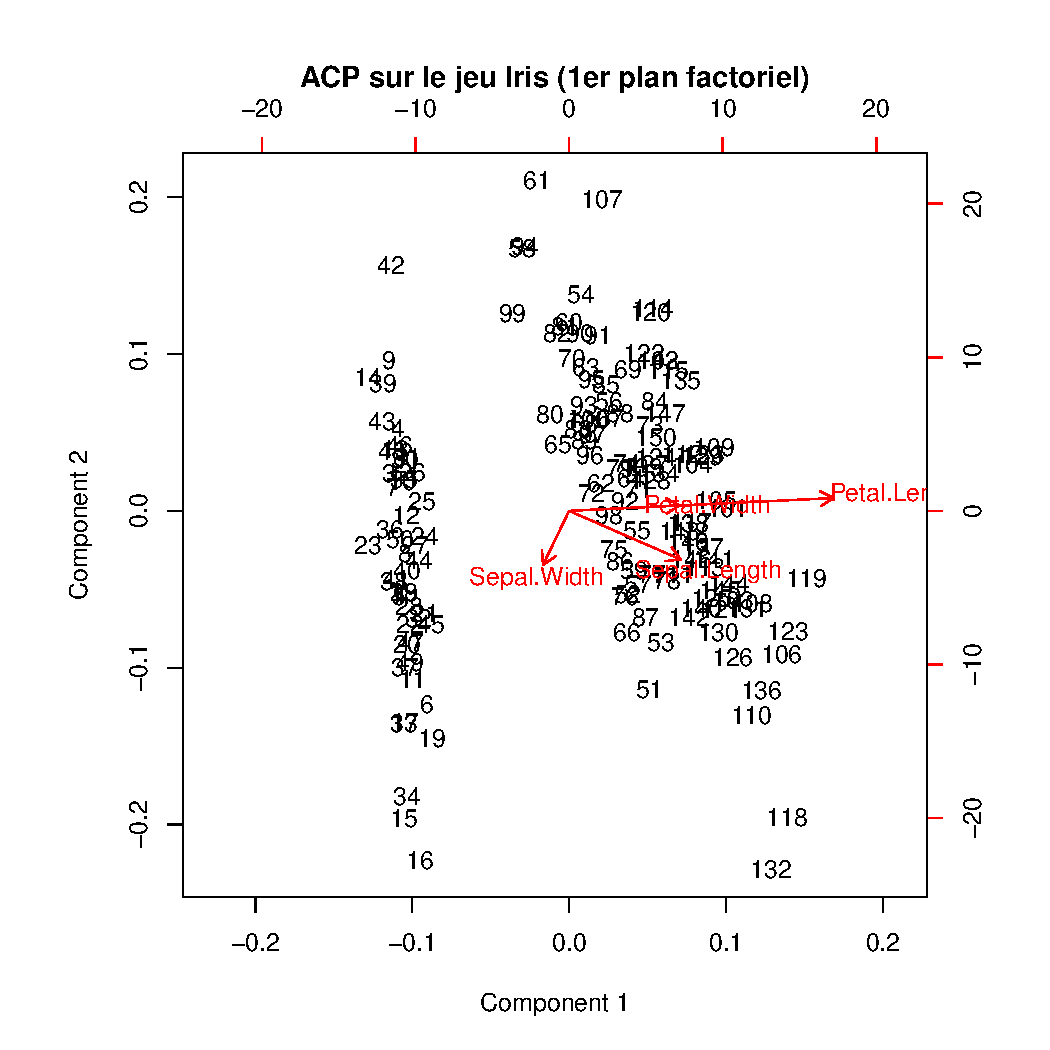
\includegraphics[width=\textwidth]{../plots/E1Q1ACPiris.pdf}
    \caption{Représentation du jeu de données Iris dans le premier plan factoriel via ACP}
\end{center}
\end{figure}
\newpage
\paragraph{Interprétation}
Cette représentation nous permet de distinguer deux groupes principaux d'invididus, répartis en deux nuages de points semblant déterminés principalement par les caractéristiques \verb+Petal.length+ et \verb+Petal.width+.
\newpage
\paragraph{Représentation dans le premier plan factoriel - Différenciation des espèces via l'ajout de couleur}
Afin de mieux visualiser les espèces, effectuons la représentation du même dataset, selon la même méthode, en différenciant les espèces via l'ajout de couleurs.
\begin{figure}[ht!]
\begin{center}
    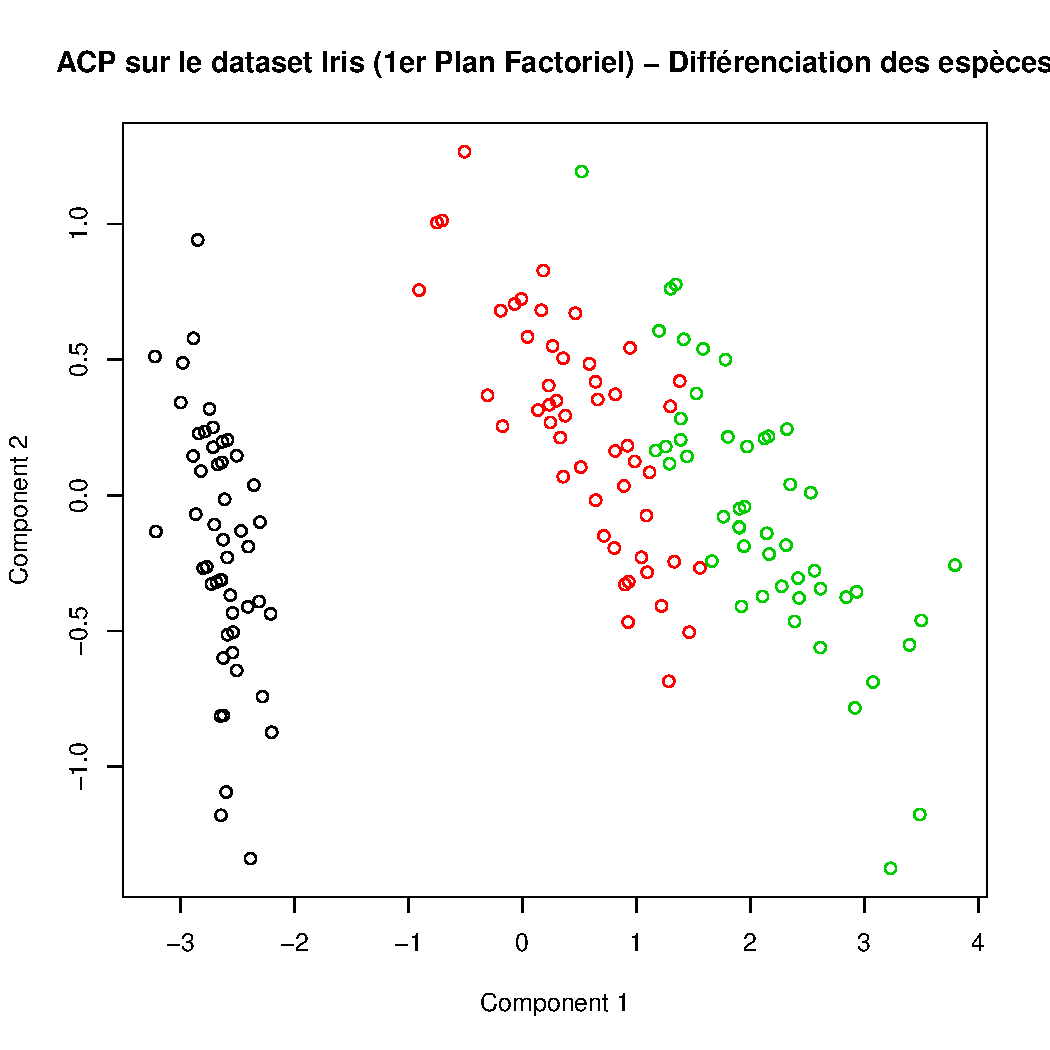
\includegraphics[width=\textwidth]{../plots/E1Q1_2_ACPiris.pdf}
    \caption{Représentation du jeu de données Iris dans le premier plan factoriel via ACP et ajout de couleurs pour différencier les espèces}
\end{center}
\end{figure}
\paragraph{Interprétation}
Cette représentation met en exergue le fait que les individus de deux espèces \textbf{différentes} forment un \textbf{et un seul} nuage de points plutôt homogène. Nous pouvons ainsi craindre que cela nous pose problème par la suite, lorsqu'il s'agira d'effectuer le clustering des Iris.
\newpage
\section{Analyse descriptive du jeu de de données Crabs2}
\paragraph{Introduction}
Le jeu de données Crabs est un jeu de données standard de R décrivant 5 mesures morphologiques sur 200 crabes mâle, femelle et bleu et orange des espèces Leptograpsus variegatus collectés à Fremantle, en Australie. Nous étudions tout d'abord les caractéristiques générales du jeu de données.
\paragraph{Représentation dans le premier plan factoriel - Pas de différenciation en fonction de l'espèce}
De la même manière que nous l'avons effectué pour les Iris, intéressons nous tout d'abord à la représentation des crabs dans le premier plan factoriel, sans différenciation de l'espèce.
\begin{figure}[ht!]
\begin{center}
    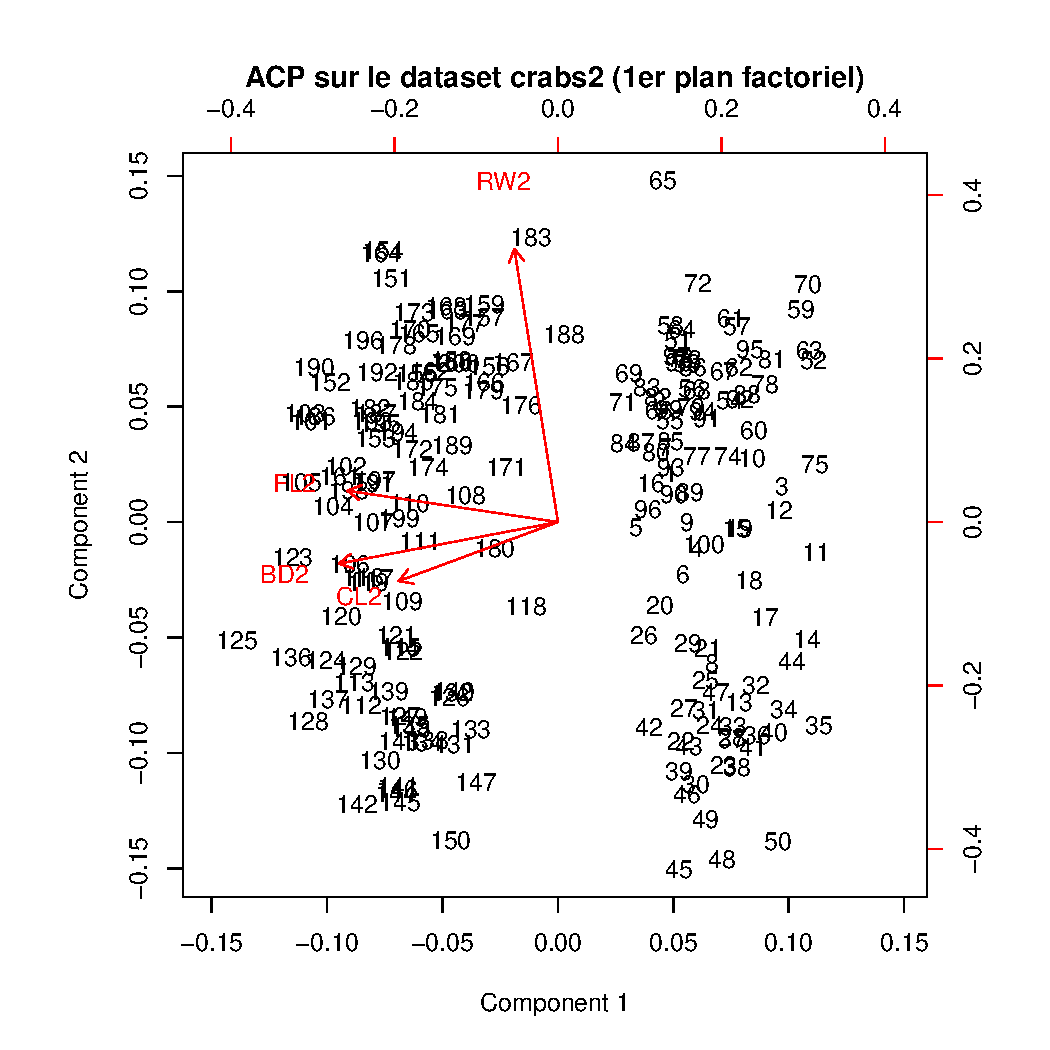
\includegraphics[width=\textwidth]{../plots/E1Q2_ACPcrabs.pdf}
    \caption{Représentation du jeu de données crabs2 dans le premier plan factoriel via ACP}
\end{center}
\end{figure}
\newpage
\paragraph{Interprétation}
Cette représentation nous permet de distinguer deux nuages de points principaux. En regardant ces nuages de points principaux, on peut deviner qu'il existe au sein des nuages plusieurs espèces d'individus : en effet chacun des nuages semble être plus concentré en deux points.
\paragraph{Représentation dans le premier plan factoriel - Différenciation des espèces via l'ajout de couleur}
Afin de mieux visualiser les différentes espèces, effectuons la représentation du même dataset, selon la même méthode, en différenciant les espèces via l'ajout de couleurs.
\begin{figure}[ht!]
\begin{center}
    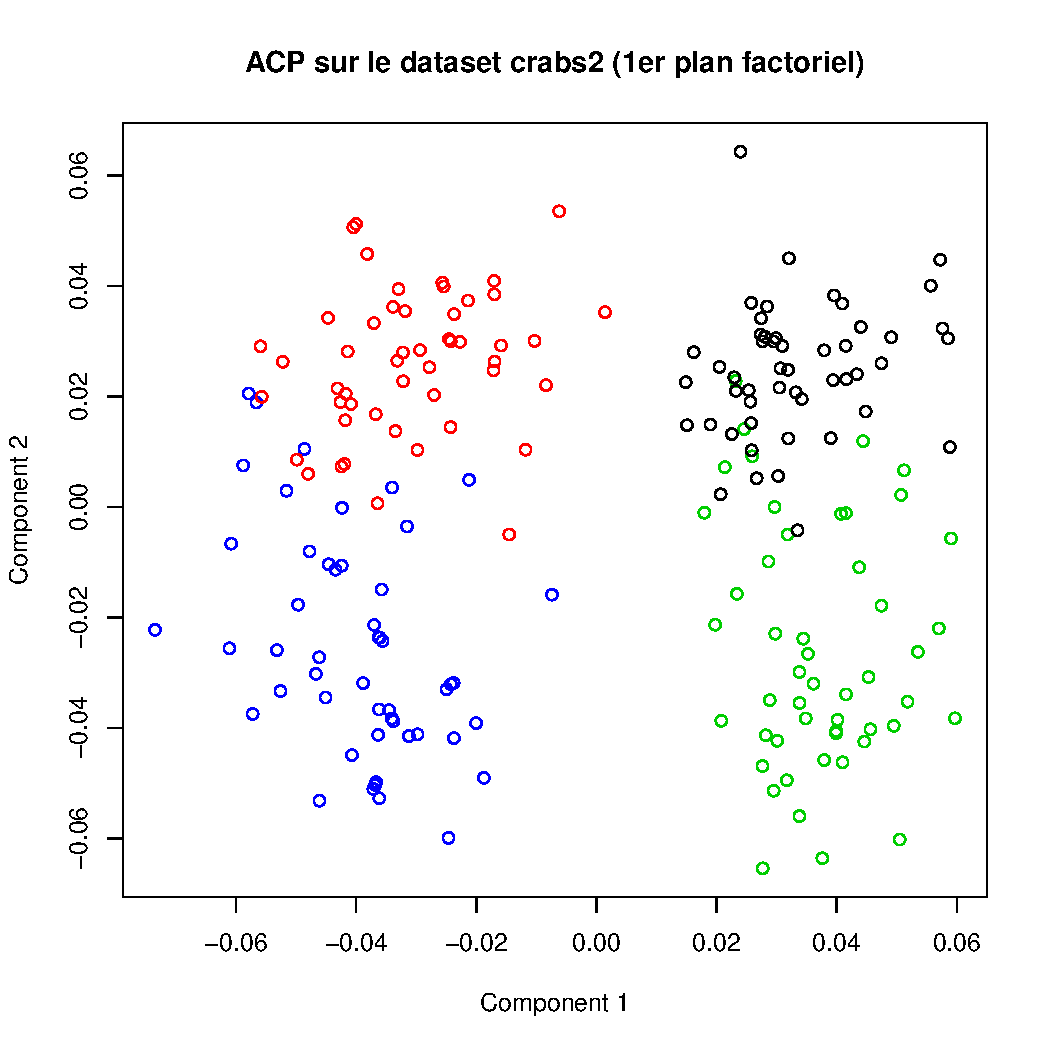
\includegraphics[width=\textwidth]{../plots/E1Q2_2_ACPcrabs.pdf}
    \caption{Représentation du jeu de données crabs dans le premier plan factoriel via ACP et ajout de couleurs pour différencier les espèces}
\end{center}
\end{figure}
\paragraph{Interprétation}
De la même manière que pour les Iris, la coloration des crabs en fonction de leur espèce met en lumière la présence au sein d'un même nuage d'individus appartenant à des catégories différentes. Nous obtenons ainsi deux nets nuages de points, au sein desquels nous retrouvons à chaque fois deux catégories d'individus. Encore une fois cela nous laisse supposer que nous pourrions être confrontés à quelques difficultés au moment de la classification.
\newpage
\section{Analyse descriptive du jeu de de données Mutations}
\paragraph{Introduction}
Nous ne travaillons plus cette fois sur des jeux de données contenant des caractéristiques morphologiques d'individus, mais à partir d'un dataset de dissimilarité entre individus. L'objectif de cette question est en quelque sorte de nous montrer qu'il existe une représentation nous permettant de visualiser les individus à caractériser. Pour cela nous allons utiliser la méthode de l'AFTD, qui permet de décomposer le tableau de distances comme produit de deux matrices. D'autres méthodes existent, telles que la méthode de Sammon, ou la méthode de Cruscan, effectuant le même traitement que l'AFTD, mais en optimisant des critères différents (minimisation des distances entre les points de la représentation / Régression isotomique / ...). Ces deux autres méthodes n'améliorent que très peu la représentation obtenue via l'AFTD, alors nous nous limiterons dans le cadre de ce TP à l'utilisation de l'AFTD.
\paragraph{AFTD - Principe}
Nous avons déjà appliqué l'ACP au cours de notre premier TP. Rappelons ici le principe de la notion d'AFTD, appliquée pour la première dans ce TP. L'AFTD peut être vue comme un équivalent de l'ACP pour des données se présentant sous la forme d'un tableau $n \times n$ de dissimilarités $\delta_{ij}$ entre $n$ individus $(i,j$ $\epsilon$ $\{1,...,n\})$ : elle calcule une représentation multidimensionnelle de ces individus (dont le tableau de dissimilarités ne donne qu'une description implicite) dans un espace euclidien de dimension $p \le n$. Cette représentation est exacte lorsque les dissimilarités sont des distances euclidiennes.
\paragraph{Dataset Mutations}
Etant donné qu'il s'agit de la première fois que nous travaillons avec ce dataset, prenons le temps de le décrire en quelques lignes. Ce dataset vient de l'étude d'une molécule de protéine, Cytochrome C, accomplissant une même fonction au sein de l'organisme de chacune des espèces étudiées dans le dataset. Le tableau de dissimilarités ainsi étudié est donc basé sur la dissimilarité de la structure de cette molécule d'une espèce à l'autre.
\paragraph{Représentation euclidienne des données par AFTD}
Nous souhaitons dans un premier temps calculer une représentation euclidienne des données par AFTD. Pour cela nous allons appliquer la méthode dite de "Positionnement Multidimensionnel" (Multidimensional Scaling en anglais, nous utiliserons donc l'abréviation "MDS") à notre matrice de dissimilarité.
\begin{figure}[ht!]
\begin{center}
    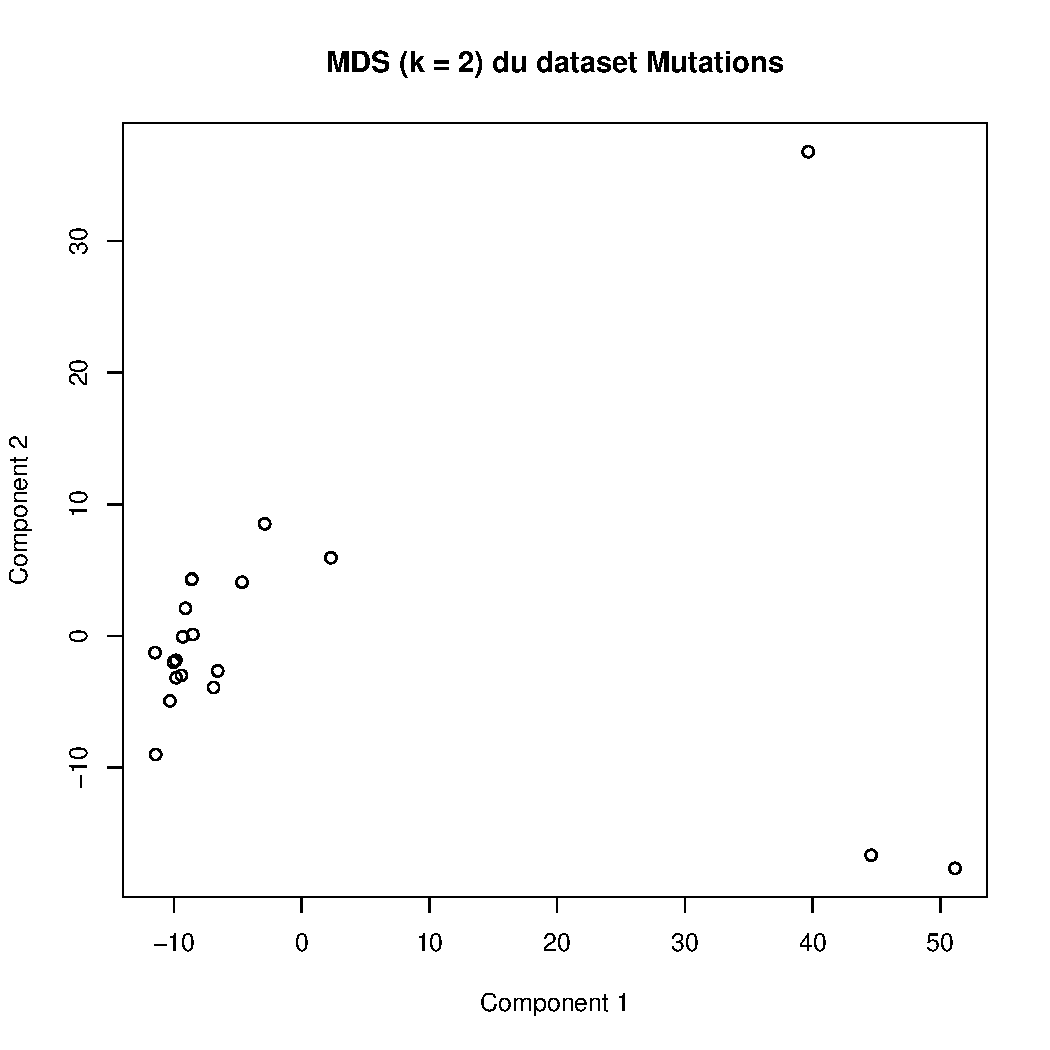
\includegraphics[width=\textwidth]{../plots/E1Q3_1.pdf}
    \caption{Multidimensional Scaling appliqué au tableau de dissimilarités du dataset Mutations (k = 2)}
\end{center}
\end{figure}
\newpage
\paragraph{Interprétation}
Cette représentation nous permet de distinguer visuellement la dissimilarité entre les différentes espèces de l'échantillon. Nous distinguons ainsi un nuage de point globalement homogène, ainsi que trois individus, en marge des autres points. Notre logique d'ingénieur (ingénieurienne ?) nous suggère donc que lors de notre classification, nous aurons une différence très nette entre les individus appartenant au nuage de point, et ceux qui sont éloignés du nuage de points. Parmi ceux éloignés du nuage de points, deux seraient relativement similaires tandis que le troisième se retrouverait relativement esseulé (ça fait beaucoup de "relativements" n'est ce pas ?)
\paragraph{Qualité de la représentation}
Cette représentation n'est pas une représentation tirée de données "brutes". Il est donc nécessaire d'en évaluer la qualité. Le tracé d'un diagramme de Shepard nous permet d'évaluer la qualité de notre représentation.
\begin{figure}[ht!]
\begin{center}
    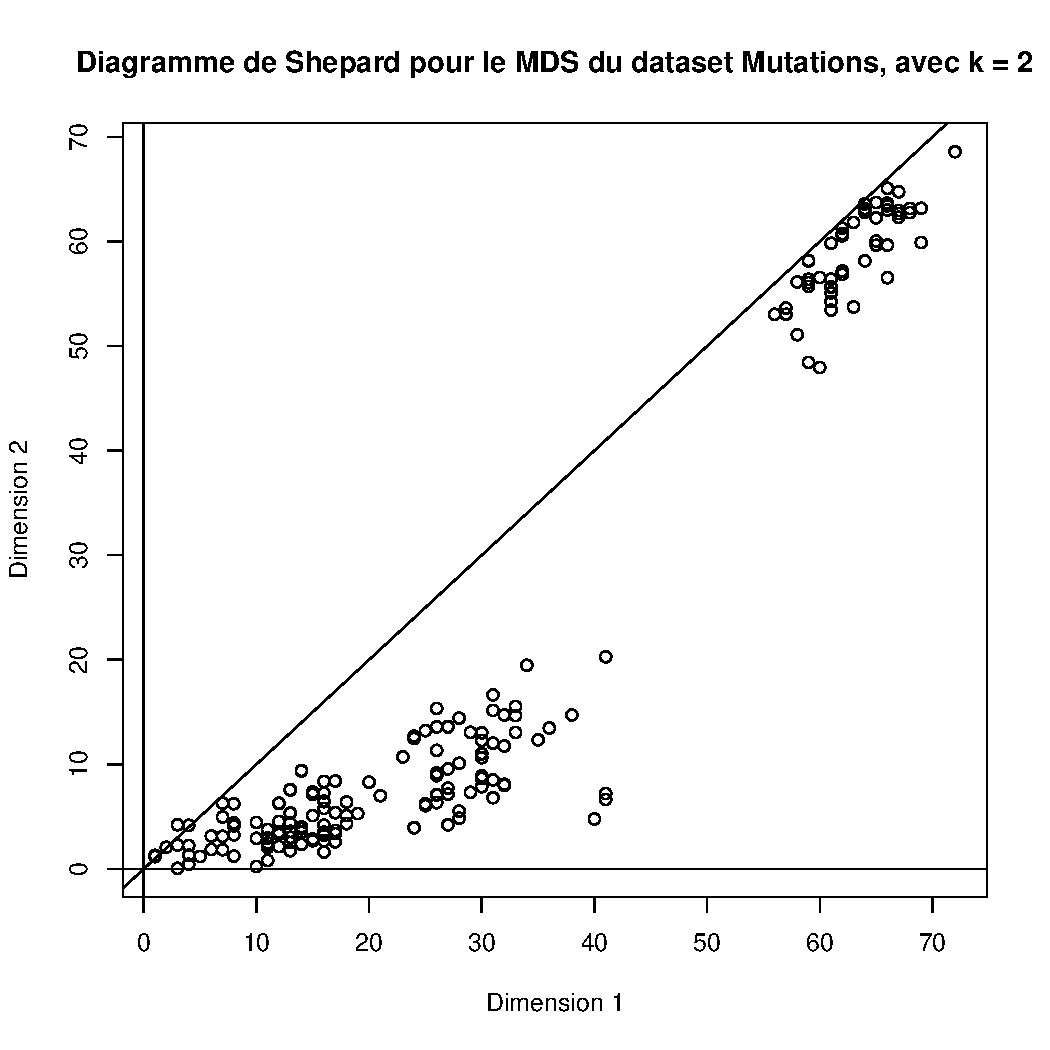
\includegraphics[width=\textwidth]{../plots/E1Q3_SHEPm.pdf}
    \caption{Diagramme de Shepard pour le Multidimensional Scaling effectué sur le dataset Mutations avec le paramètre k = 2}
\end{center}
\end{figure}
\paragraph{Interprétation}
La qualité de notre réprésentation MDS peut être jugée en fonction de la propension qu'ont les points du diagramme de Shepard résultant à s'aligner sur une droite (ici la droite $x = y$). Dans notre cas, le diagramme résultant lorsque nous paramètrons notre MDS à k = 2 présente des points plutôt dispersés, ce qui nous laisse penser que la qualité de notre représentation n'est pas optimale.
\paragraph{Tests en augmentant la valeur du nombre de variables utilisées pour la représentation euclidienne des données}
Nous décidons de réitérer l'opération en augmentant le nombre $d$ de variables utilisées pour la représentation euclidienne de nos données par AFTD.
\begin{figure}[ht!]
\begin{center}
    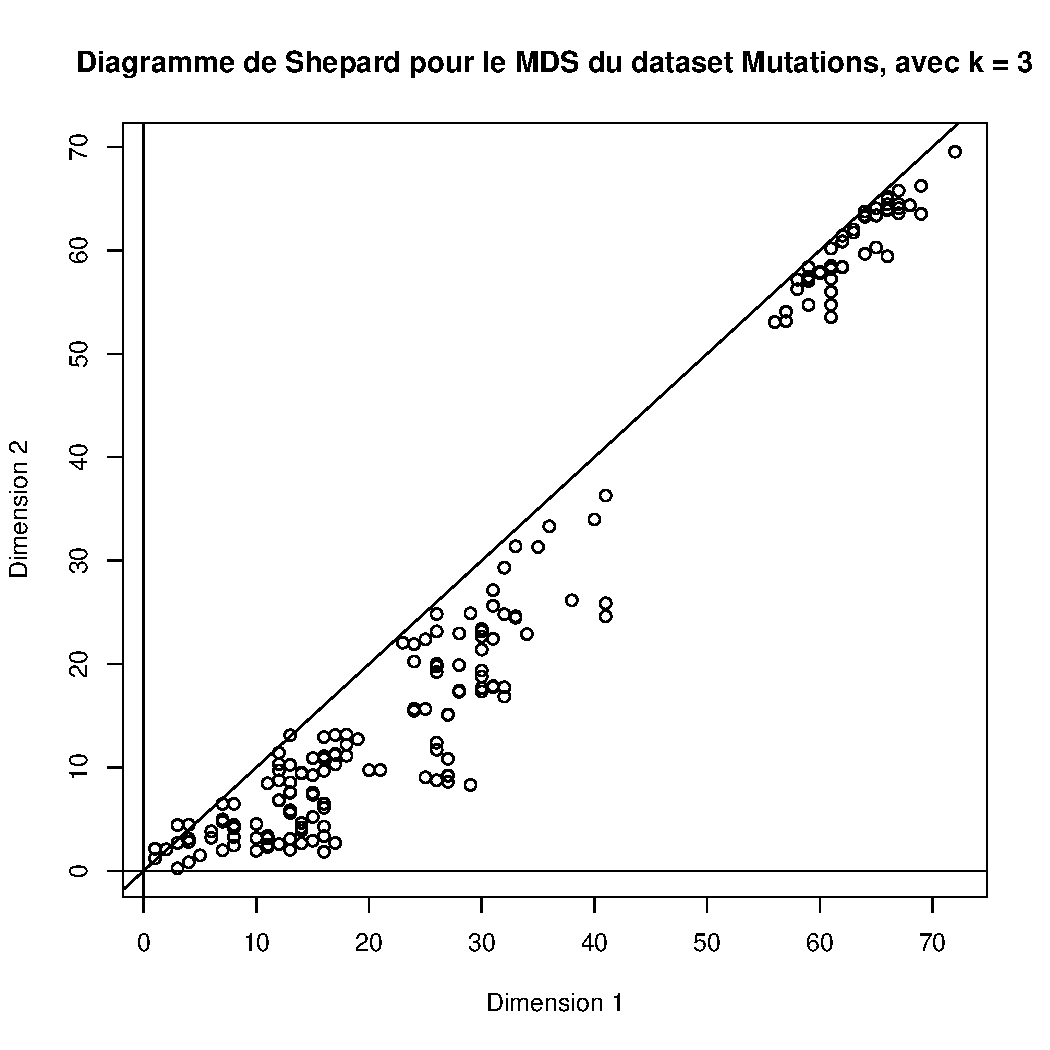
\includegraphics[width=\textwidth]{../plots/E1Q3_SHEP3m.pdf}
    \caption{Diagramme de Shepard pour le Multidimensional Scaling effectué sur le dataset Mutations avec le paramètre k = 3}
\end{center}
\end{figure}
\begin{figure}[ht!]
\begin{center}
    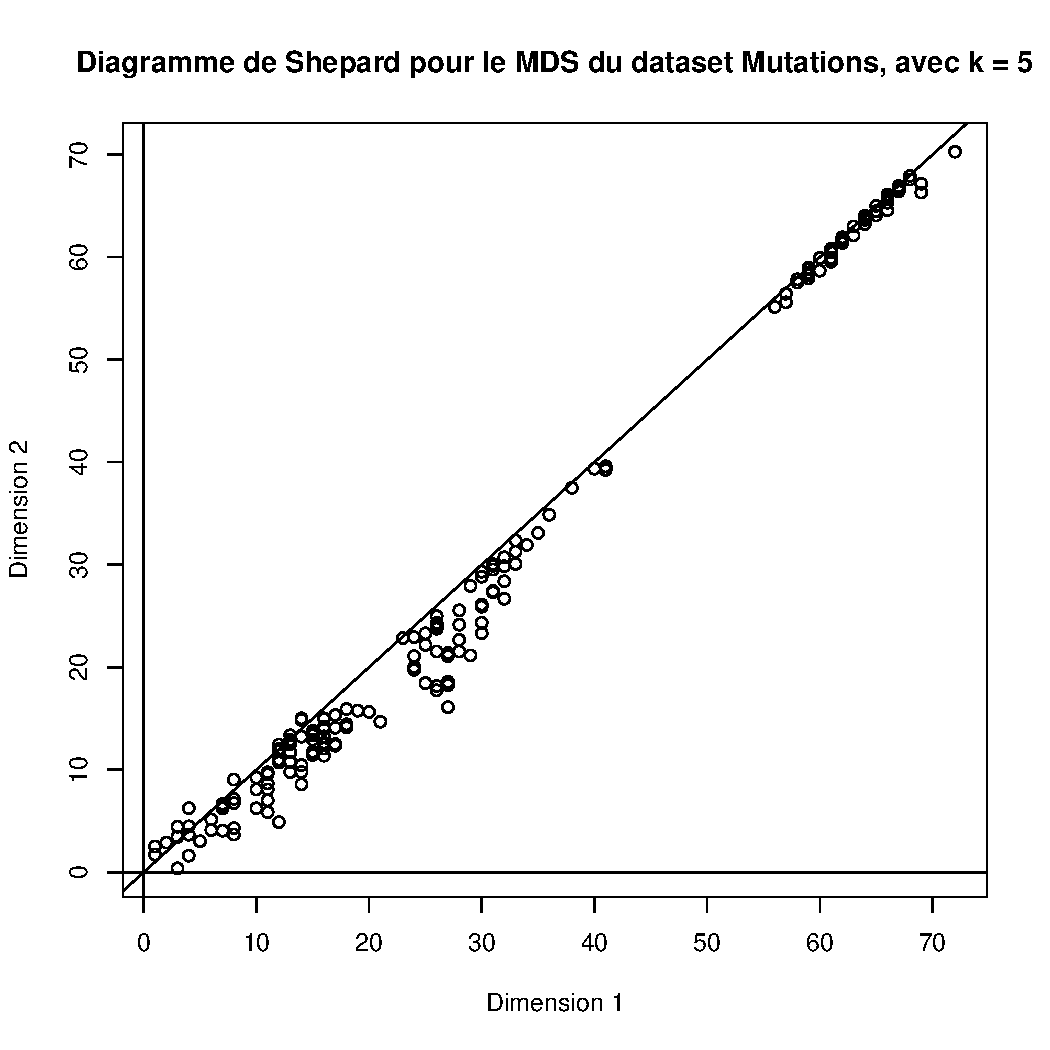
\includegraphics[width=\textwidth]{../plots/E1Q3_SHEP5m.pdf}
    \caption{Diagramme de Shepard pour le Multidimensional Scaling effectué sur le dataset Mutations avec le paramètre k = 5}
\end{center}
\end{figure}
\paragraph{Interprétation}
Le fait d'augmenter la valeur du nombre de variables utilisées pour la réprésentation de nos données agit très clairement sur la qualité de notre représentation. Il est donc nécessaire d'utiliser le bon nombre de variables afin d'obtenir un MDS de qualité optimale.
\newpage
\chapter{Exercice 2 - Classification Hiérarchique}
\section{Introduction}
\paragraph{Objectif}
L'objectif de ce second exercice est de se familiariser avec les méthodes de classification hiérarchique, notamment la classification hiérarchique ascendante et la classification hiérarchique descendante.
\paragraph{Classification hiérarchique}
L'objectif de la classification hiérarchique est de construire une hiérarchie indicée d'un ensemble $\Omega$ sur lequel on connait une mesure de dissimilarité $d$ telle que les points les plus proches soient regroupés dans les classes de plus petit indice.
\paragraph{Classification hiérarchique descendante}
Dans le cas de la classification hiérarchique descendante, on divise l'ensemble $\Omega$ en classes, puis on recommence sur chacune de ces classes et ainsi de suite jusqu'à ce que les classes soient réduites à des singletons. Par exemple, on peut découper les classes par dichotomie successives, chacune de ces dichotomies étant définie par la vérification ou non d'une propriété.
\paragraph{Classification hiérarchie ascendante}
Cette fois on part de la partition de $\Omega$ où chaque classe est un singleton. On procède alors par fusion successive des classes qui se "ressemblent" jusqu'à obtenir une seule classe, c'est-à-dire l'ensemble $\Omega$ lui-même. Cette procédure est beaucoup plus utilisée que la classification hiérarchique descendante.
\paragraph{Application - Classification ascendante}
Utilisons donc la fonction \verb+hclust+ de R afin d'obtenir une classification hiérarchique ascendante de notre dataset Mutations.
\begin{figure}[ht!]
\begin{center}
    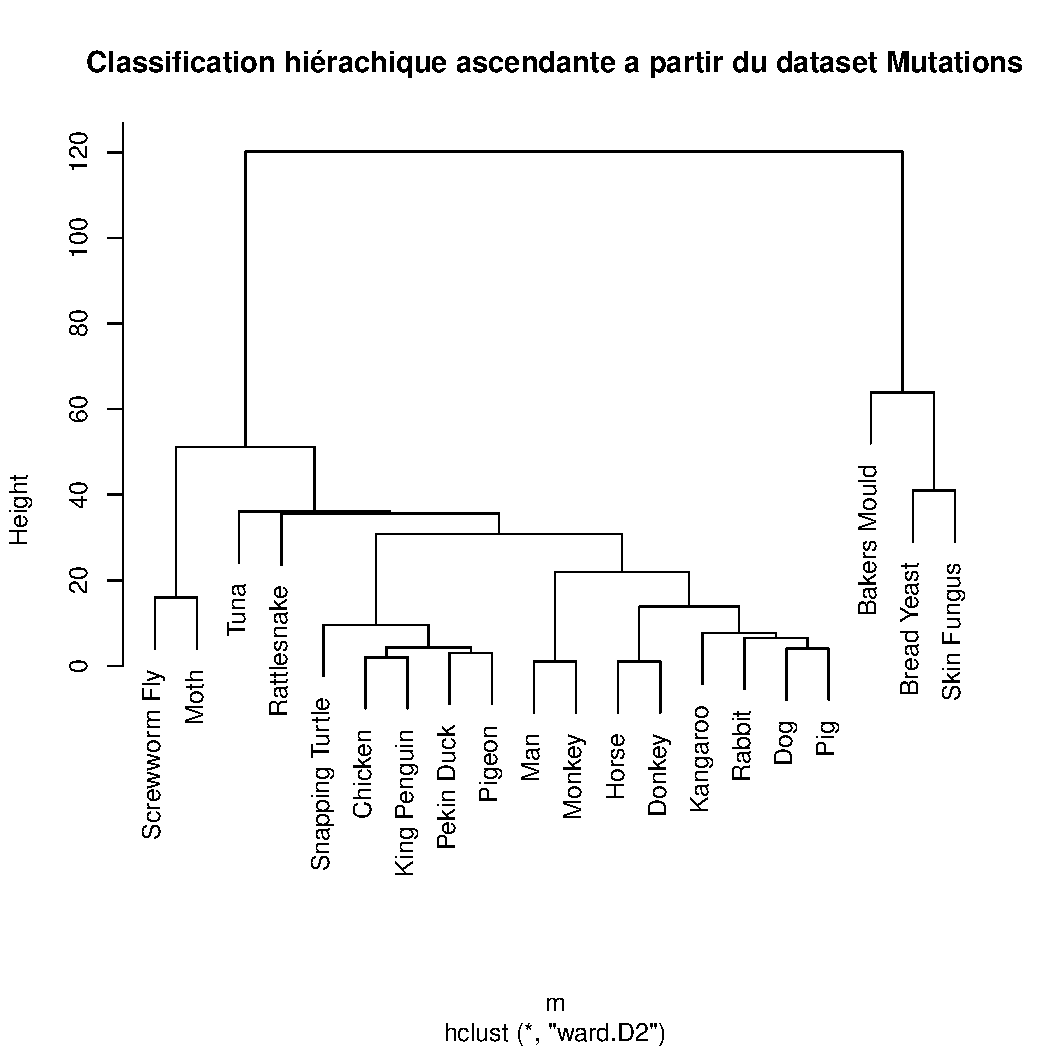
\includegraphics[width=\textwidth]{../plots/E2Q1_CLUSTm.pdf}
    \caption{Classification hiérarchique ascendante du dataset Mutations}
\end{center}
\end{figure}
\newpage
\paragraph{Interprétation}
La classification hiérarchique ascendante du dataset semble confirmer les hypothèses que nous avions faites au moment de la réalisation de l'AFTD. Nous retrouvons ces deux classes principales : celle de notre précédent nuage de points, et celle contenant les points esseulés, et nous retrouvons également la séparation entre le groupe de deux points, et les point seul, lorsque l'on "descend" dans notre classification hiérarchique. En descendant encore plus (toujours en se referrant à la hauteur, \verb+height+), nous nous apercevons que certaines espèces appartenant au nuage de point principal, sont tout de même assez différente de la "masse" d'espèces composant le nuage. Nous pouvons mettre cela en relation avec le fait que malgré que le nuage soit globalement plutôt homogènes, certains individus se détachaient plus que les autres de cette homogénéité.
\newpage
\section{Classification hiérarchique ascendante - Dataset Iris}
\paragraph{Introduction}
Nous souhaitons effectuer la classification hiérarchique ascendante des Iris. Pour cela, il est à noter que nous transformons notre dataset en tableau de dissimilarité via la fonction \verb+dist+ de R avant de la passer à la fonction \verb+hclust+.
\paragraph{Classification}
Répétons donc l'opération de classification sur le dataset d'Iris.
\begin{figure}[ht!]
\begin{center}
    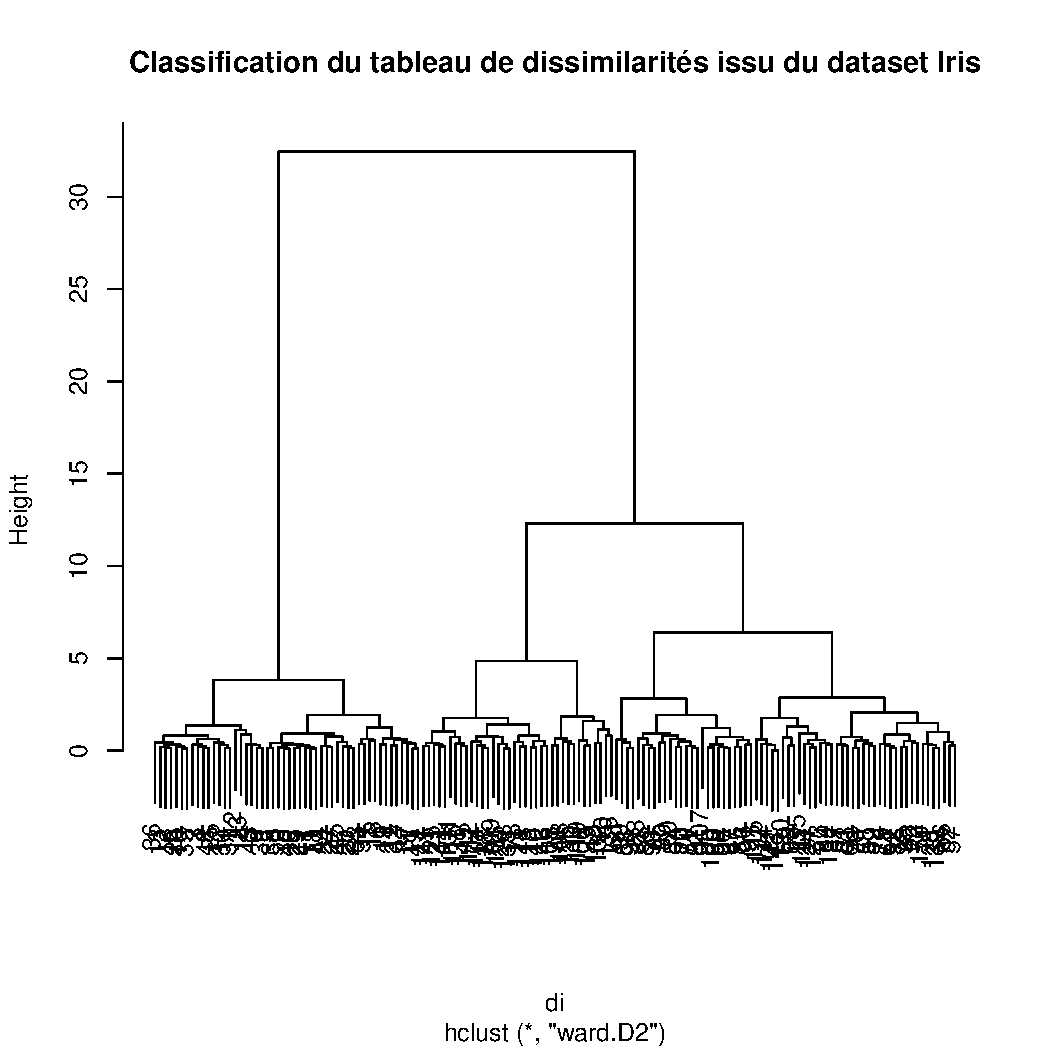
\includegraphics[width=\textwidth]{../plots/E2Q2_cdi.pdf}
    \caption{Classification hiérarchique ascendante du tableau de dissimilarités issu du dataset Iris}
\end{center}
\end{figure}
\newpage
\paragraph{Interprétation}
De nouveau, la classification hiérarchique ascendante confirme les hypothèses que nous avions pu faire au cours de notre étude du dataset Iris via l'ACP : il en ressort, lorsque l'on reste à une hauteur conséquente, qu'il est extrêmement facile de distinguer deux classes principales d'Iris, et qu'en "s'enfoncant" par la suite légèrement dans notre classification, que l'une de ces classes peut être en réalité divisée en deux sous-classes principales. Nous retrouvons ainsi nos 3 espèces d'origine.
\newpage
\section{Classification hiérarchique descendante - Dataset Iris}
\paragraph{Classification}
Pour finir, réalisons la classification hiérarchique descendante des données du dataset Iris, au moyen de la fonction \verb+diana+ de la library cluster de R.
\begin{figure}[ht!]
\begin{center}
    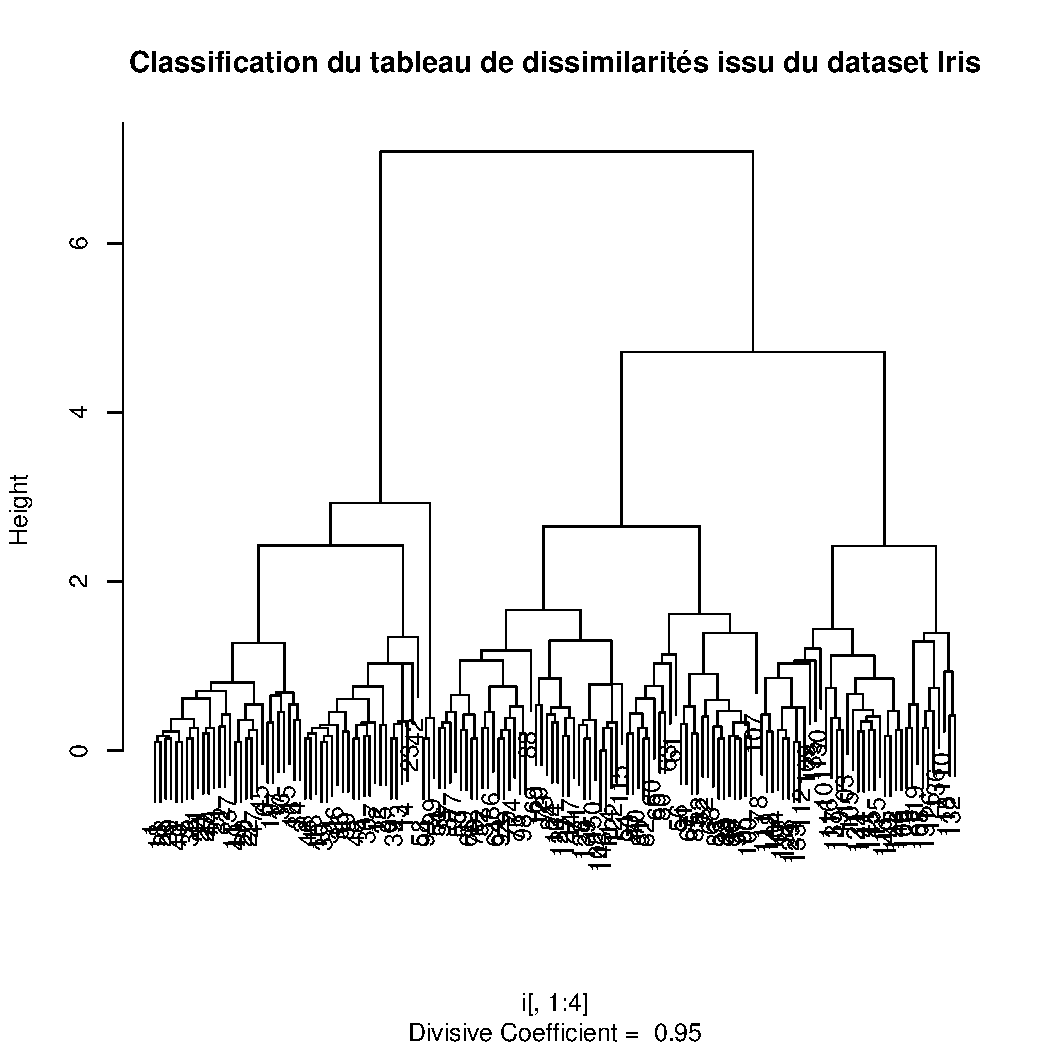
\includegraphics[width=\textwidth]{../plots/E2Q3_diani.pdf}
    \caption{Classification hiérarchique descendante du tableau de dissimilarités issu du dataset Iris}
\end{center}
\end{figure}
\newpage
\paragraph{Interprétation}
Nous retrouvons encore une fois notre division en deux classes si l'on s'en tient à une certaine hauteur dans la classification, ou trois, si l'on "descend" un peu. Bien que la méthode de classification utilisée soit différente de la classification hiérarchique ascendante, les deux partitionnements trouvés sont très similaires et il en va de même pour la représentation.
\newpage
\chapter{Exercice 3 - Méthode des centres mobiles}
\section{Application de la méthode des centres mobiles au dataset Iris}
\subsection{Introduction}
\paragraph{Méthode des centres mobiles}
La méthode des centres mobiles, aussi connue sous le nom de méthode de réallocation-centrage ou des k-means (MacQueen, 1967) est la méthode de classification de référence lorsque l'ensemble à classifier est mesuré par p variables continues. L'ensemble $\Omega$ à classifier correspond donc à un ensemble de $n$ individus mesurés par $p$ variables quantitatives.
\paragraph{Algorithme des centres mobiles}
L'algorithme des centres mobiles, utilisé pour effectuer la classification, peut être résumé comme suit. L'algorithme commence par tirer au hasard $g$ points de $\Omega$ qui forment les centres initiaux des $g$ classes. Par la suite, tant qu'il n'y a pas convergence, l'algorithme construit la partition suivante en affectant chaque point de $\Omega$ à la classe dont il est le plus près du centre (en cas d'égalité, l'affectation se fait à la classe de plus petit indice) puis calcule les centres de gravité de la partition qui vient d'être calculée, qui deviennent les centres de la partition suivante.
\subsection{Objectif}
L'objectif de cet exercice est d'appliquer la méthode des k-means aux différents datasets étudiés précédemment et d'en interpréter les résultats.
\subsection{Q1 - Partitionnement en 2, 3 et 4 classes}
\paragraph{Partitionnement en 2, 3 et 4 classes}
Nous utilisons donc dans un premier temps la méthode \verb+k-means+ de R afin de partitionner successivement le jeu de données Iris en 2, 3 et 4 classes.
\begin{figure}[ht!]
\begin{center}
    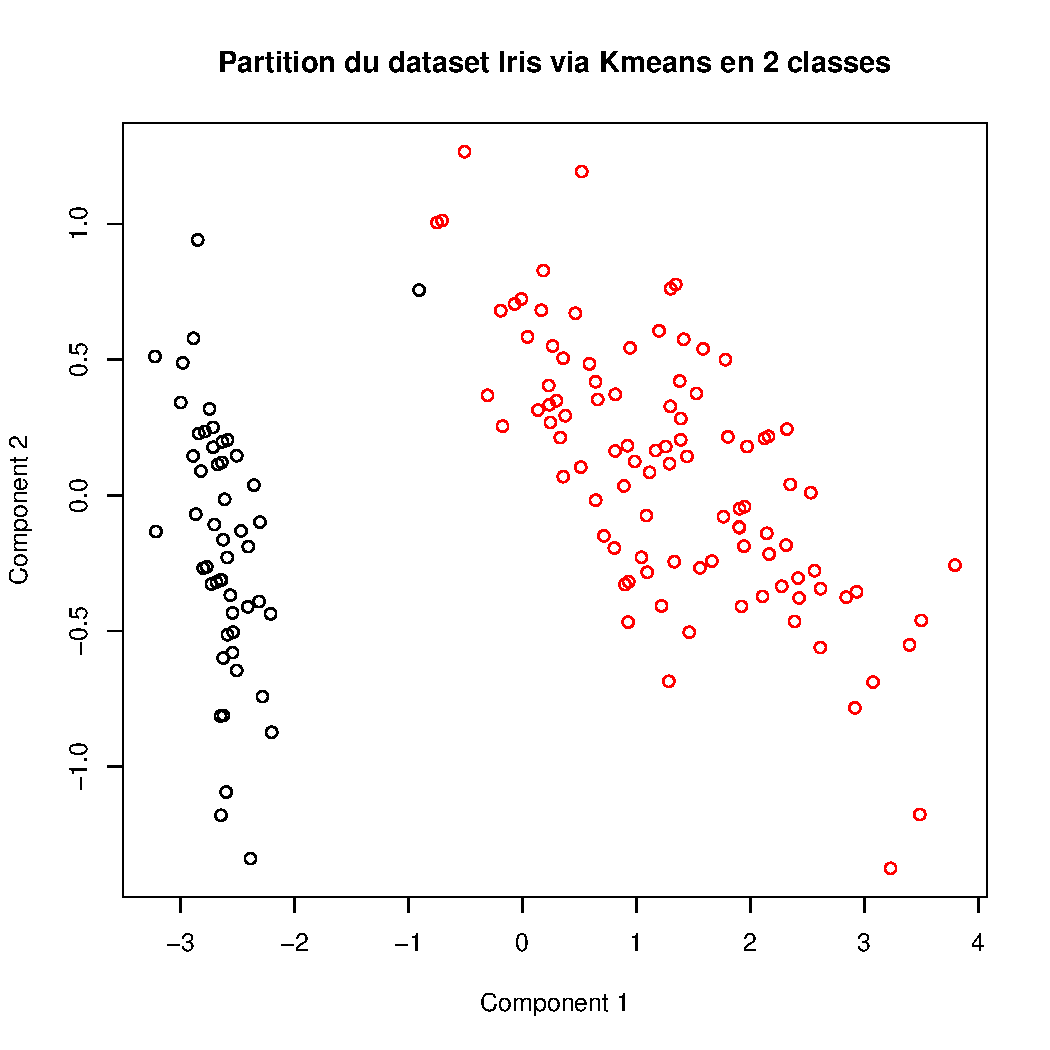
\includegraphics[width=\textwidth]{../plots/E3Q1_ki2.pdf}
    \caption{Partitionnement du dataset Iris en 2 classes (représenté via ACP)}
\end{center}
\end{figure}

\paragraph{Interprétation}
En partitionnant le dataset en deux classes, nous obtenons le résultat le plus intuitif : les deux nuages de point sont bien caractérisés par une couleur différente (et non pas les deux classes confondues au sein du nuage de droite). Afin de vérifier la cohérence de la classification nous utilisons cependant la réprésentation \verb+pairplot+ donnant le résultat suivant.
\begin{figure}[ht!]
\begin{center}
    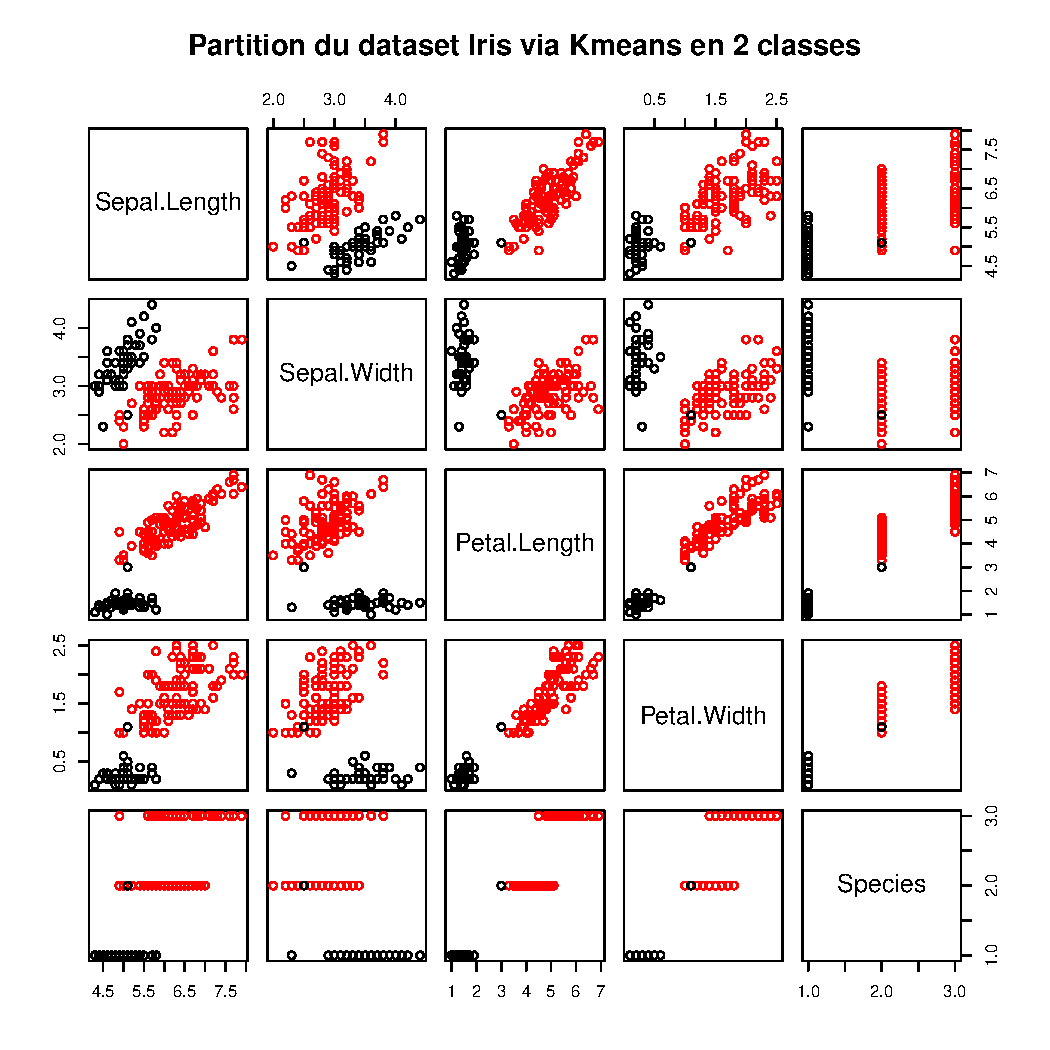
\includegraphics[width=\textwidth]{../plots/E3Q1_ki2_2.pdf}
    \caption{Partitionnement du dataset Iris en 2 classes (représenté via Pairplot)}
\end{center}
\end{figure}
\newpage
\paragraph{Interprétation}
Nous remarquons grâce à cette représentation qu'effectivement, la quasi totalité des individus semblent correctement classés, c'est à dire que les individus des deux espèces les moins dissimilaires sont classés dans une première classe commune, et ceux de la classe la plus dissimilaire des deux autres sont classés dans la seconde classe. Cependant, un très faible nombre d'individus ont été classés dans une mauvaise classe.
\begin{figure}[ht!]
\begin{center}
    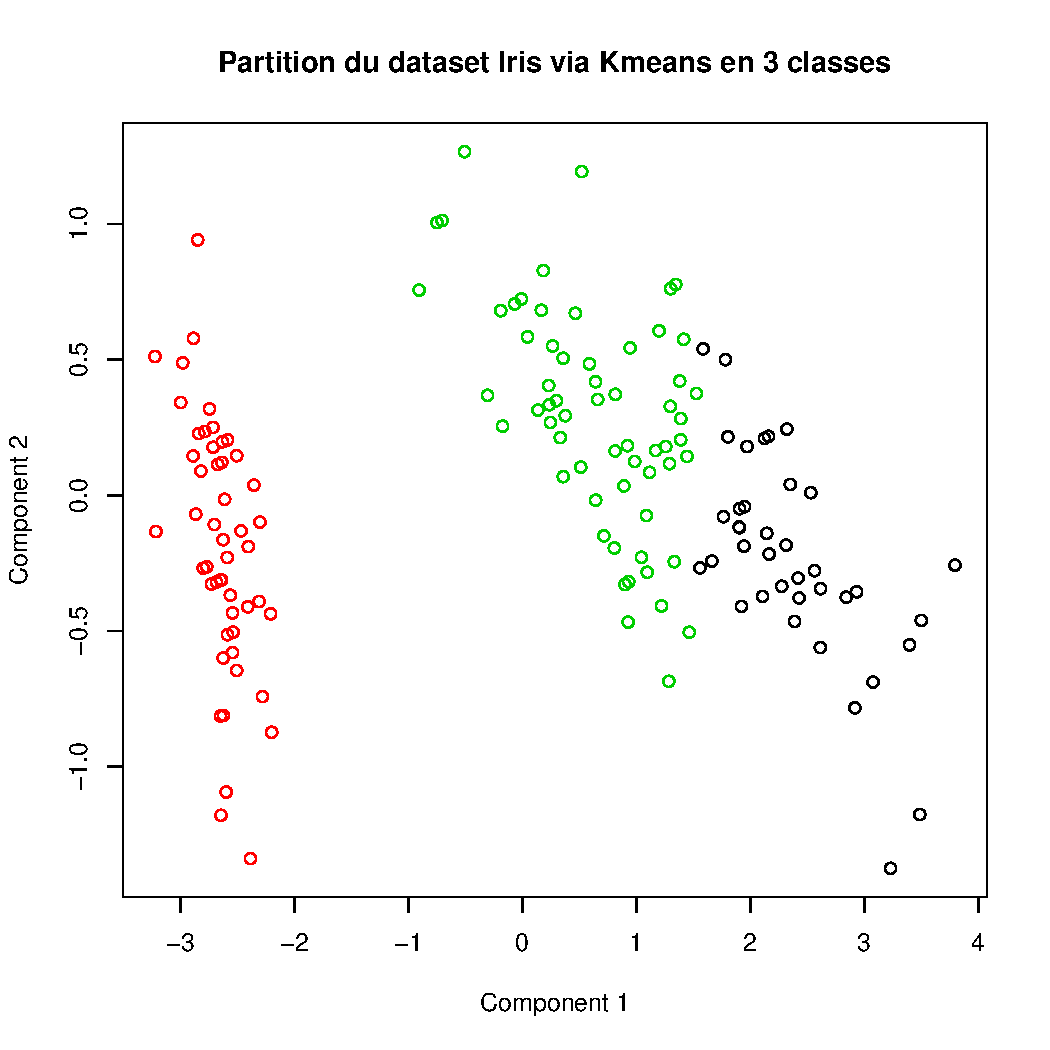
\includegraphics[width=\textwidth]{../plots/E3Q1_ki3.pdf}
    \caption{Partitionnement du dataset Iris en 3 classes (représenté via ACP)}
\end{center}
\end{figure}
\newpage
\paragraph{Interprétation}
En partitionnant le dataset en trois classes, nous obtenons le résultat le plus juste scientifiquement parlant : les individus de chacune des espèces semblent correctement classés au sein de la classe de leurs pairs. Cependant, la représentation \verb+pairplot+ met de nouveau en lumière certaines incohérences.
\begin{figure}[ht!]
\begin{center}
    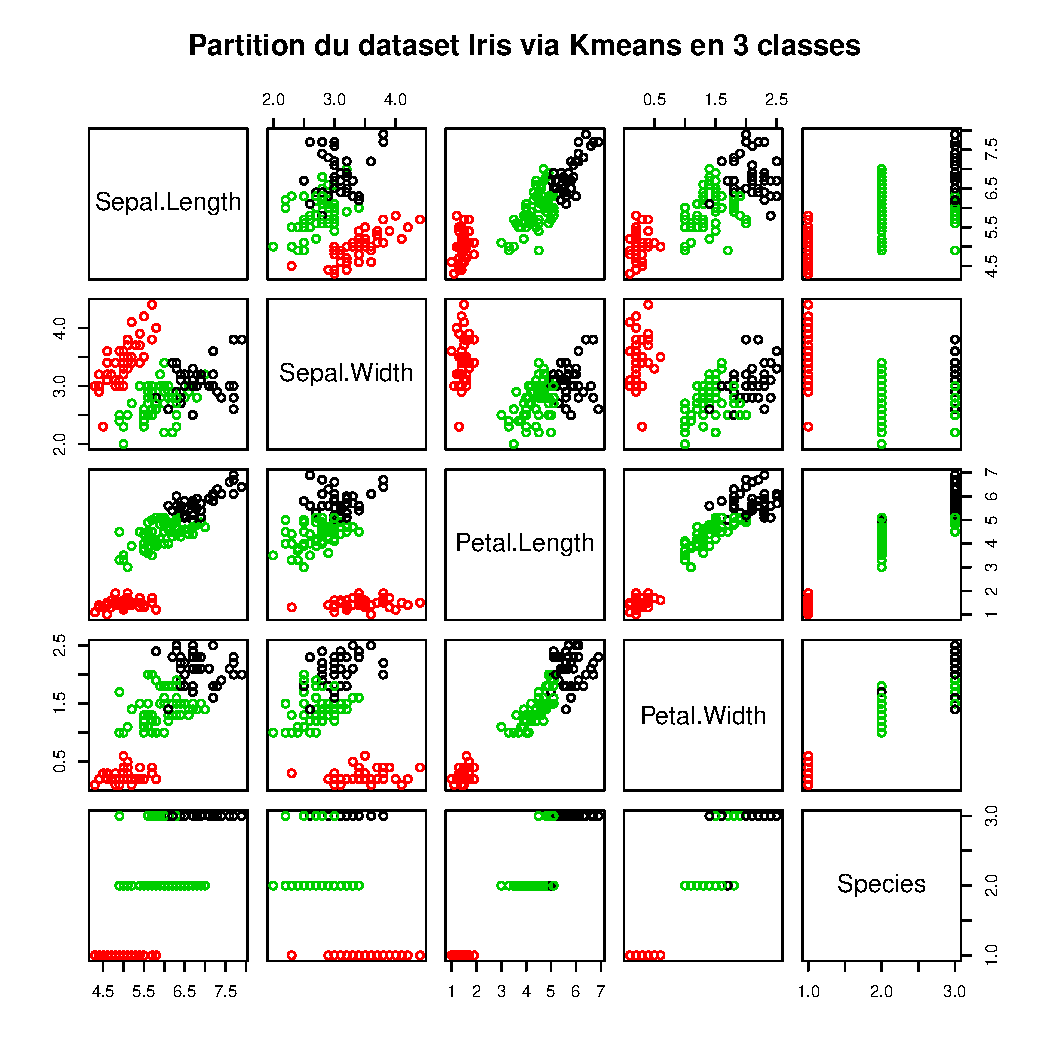
\includegraphics[width=\textwidth]{../plots/E3Q1_ki3_2.pdf}
    \caption{Partitionnement du dataset Iris en 3 classes (représenté via Pairplot)}
\end{center}
\end{figure}
\newpage
\paragraph{Interprétation}
Cette fois ci, il devient clair que même si la méthode des k-means produit de très bons résultats, elle n'est pas infaillible. Nous remarquons en effet qu'une certain nombre d'individus n'a pas été rattaché à la classe que nous aurions espéré.
\begin{figure}[ht!]
\begin{center}
    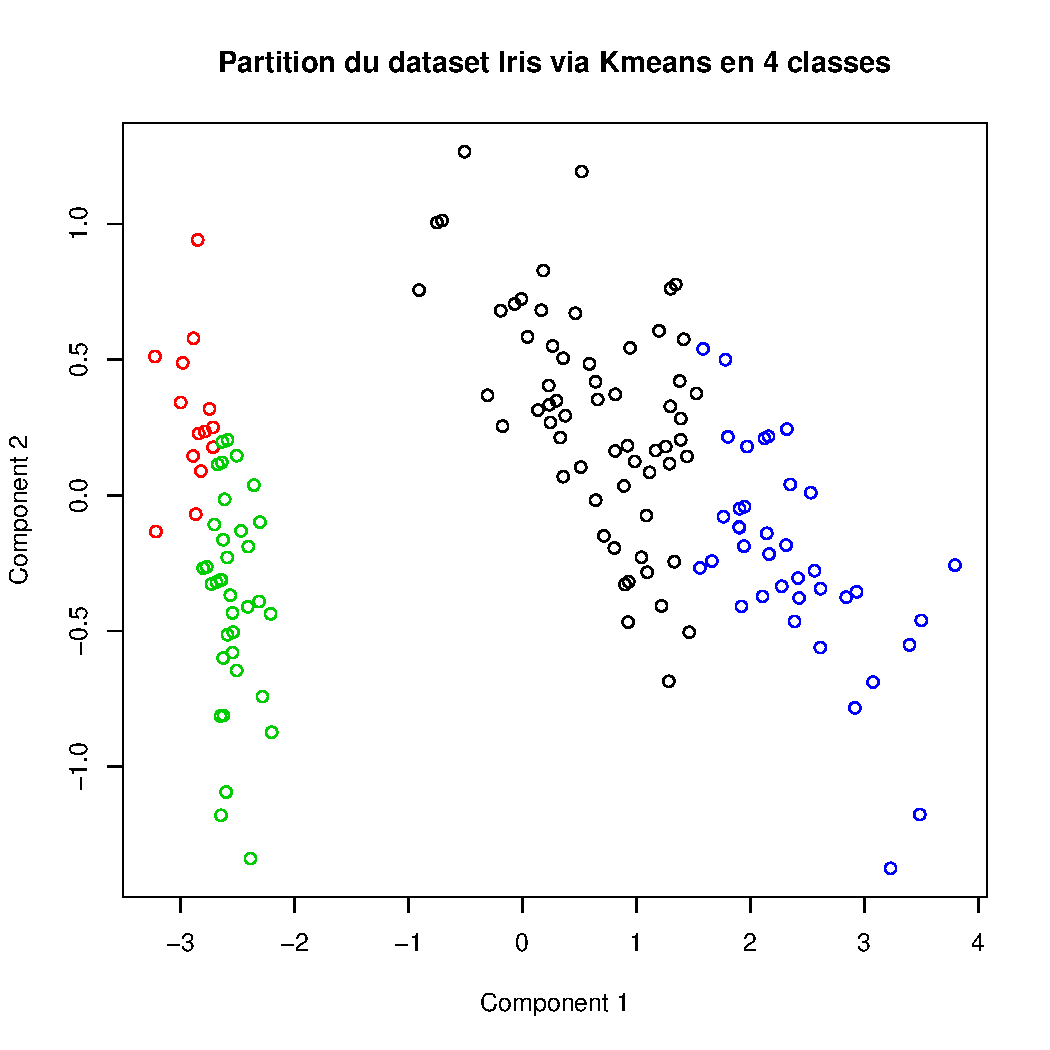
\includegraphics[width=\textwidth]{../plots/E3Q1_ki4.pdf}
    \caption{Partitionnement du dataset Iris en 4 classes (représenté via ACP)}
\end{center}
\end{figure}
\newpage
\paragraph{Interprétation}
Cette partition des Iris en 4 classes produit un résultat très similaire à la partition précédente, à la différence que le nuage d'individus de gauche a été scindé en deux classes d'individus. Nous pouvons aisément imaginer que cette séparation peut être retrouvée en descendant de 3 à 4 classes dans les classifications hiérarchiques effectuées auparavant sur le dataset Iris. Cependant, ces dernières nous ont montré qu'au delà d'un partitionnement en 3 classes, le partitionnement en plus de classes perd très vite en généralisation étant donné les faibles différences de hauteur entre un partitionnement en 3 classes et un partitionnement en plus de classes. Partitionner en 4 classes les Iris s'est donc révélé de pertinence scientifique réellement limitée.
\paragraph{Note}
L'étude du pairplot associé à ce partitionnement en 4 classes n'apporte que très peu d'informations, nous avons décidé de ne pas nous en servir.
\paragraph{Conclusion}
En conclusion, l'application de la méthode des k-means afin d'accomplir des tâches de classification non supervisée s'est révélée plutôt efficace, \textbf{CEPENDANT}, il est nécessaire de rappeler que cette méthode n'est absolumment pas infaillible, et classe parfois certains individus dans une classe non-appropriée. Notons également qu'il est \textbf{indispensable} d'évaluer la pertinence du nombre de classes choisies pour notre classification : un trop faible nombre de classe empêche la mise en exergue de spécificités de classes, tandis qu'un nombre trop élevé de classes empêche une bonne généralisation à partir des individus.
\newpage
\subsection{Q2 - Etude de la stabilité du résultat de la partition}
\paragraph{Introduction}
Nous décidons maintenant de nous intéresser à la stabilité du résultat. Pour cela nous allons répéter plusieurs fois l'opération de classification par les k-means afin de comparer les différents résultats obtenus et étudier l'évolution de l'inertie des résultats obtenus successivement.
\paragraph{Plusieurs tentatives d'utilisation de la méthode des k-means}
Pour commencer, répétons plusieurs fois la manipulation de classification en k = 3 classes des Iris.
\begin{figure}[ht!]
\begin{center}
    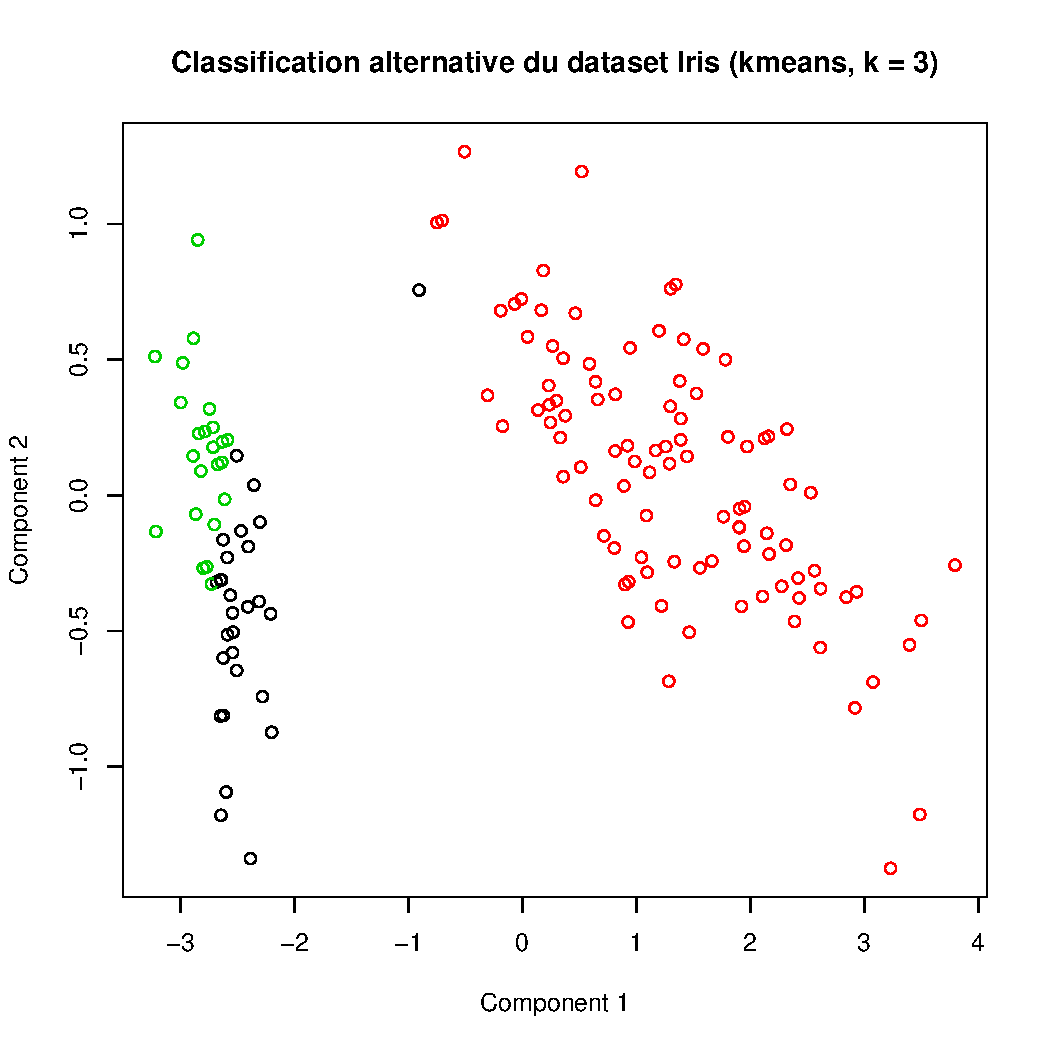
\includegraphics[width=\textwidth]{../plots/E3Q2_altCLUSi.pdf}
    \caption{Partitionnement alternatif du dataset Iris en 3 classes (représenté via ACP)}
\end{center}
\end{figure}
\begin{figure}[ht!]
\begin{center}
    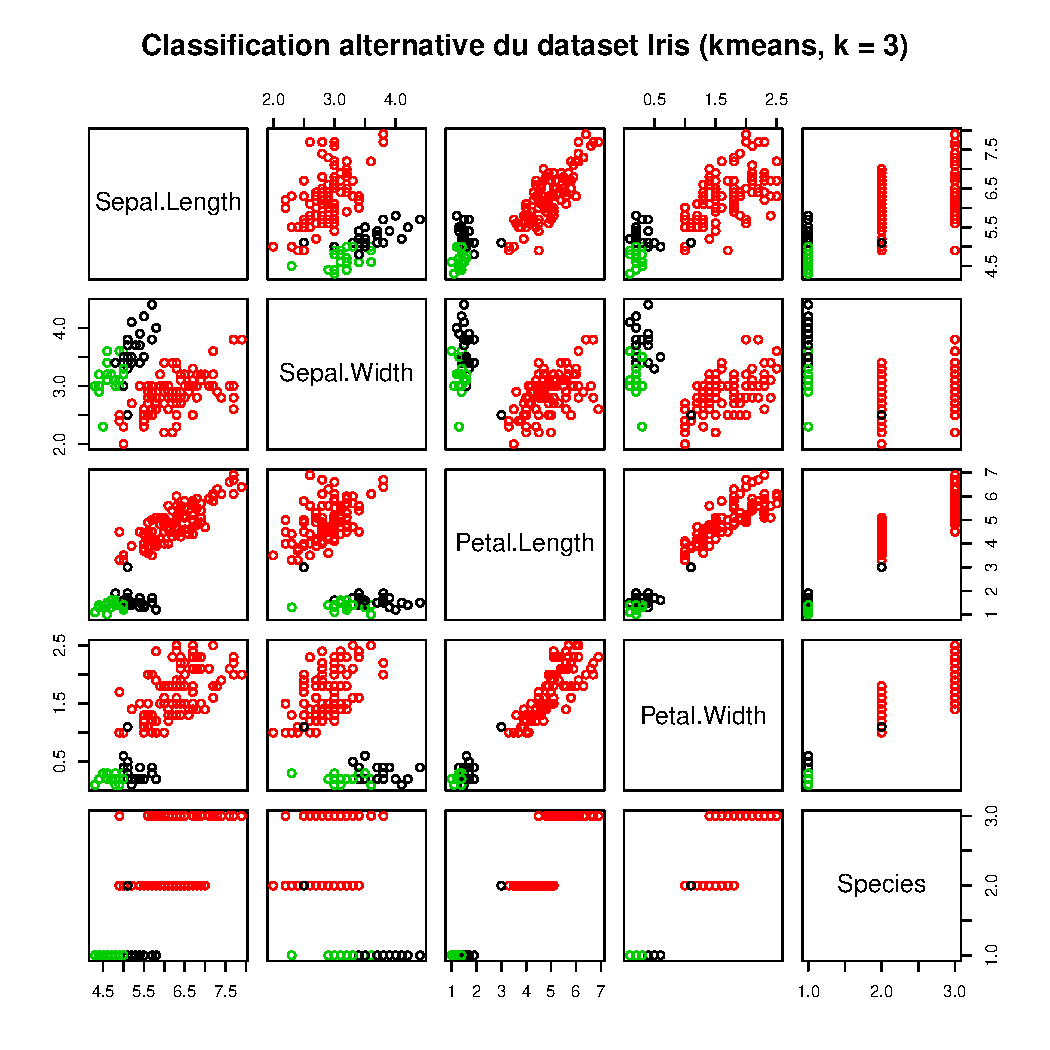
\includegraphics[width=\textwidth]{../plots/E3Q2_altCLUSi_2.pdf}
    \caption{Partitionnement alternatif du dataset Iris en 3 classes (représenté via Pairplot)}
\end{center}
\end{figure}
\newpage
\paragraph{Interprétation}
Les deux précédents plots mettent clairement en évidence que la classification des Iris en utilisant exactement la même méthode ne produit pas tout le temps les mêmes résultats. Nous observons également des différences d'inertie intra-classe entre les différents résultats de classification. Ces différences de résultat s'expliquent par le fait que l'algorithme utilisé par la méthode \verb+k-means+ n'est pas déterministe.
\newpage
\subsection{Q3 - Nombre de classes optimal}
\paragraph{Introduction - Méthode du coude}
Il n'existe pas de méthode universelle de détermination du nombre optimal de classes pour une classification donnée. Dans le cadre de ce TP, nous utilisons la méthode du coude.
\paragraph{Méthode du coude}
La méthode du coude consiste à mesurer l'évolution de la valeur d'inertie intra-classe minimale obtenue en partitionnant un ensemble en faisant varier le nombre K de classes différentes produites. L'étude de cette évolution révèle un coude, correspondant au nombre de classe à partir duquel le partitionnement de l'échantillon en plus de classe n'est plus pertinent.
\newpage
\paragraph{Calcul de l'inertie intra-classe minimale pour la classification du dataset Iris en K allant de 1 à 10 classes}
Nous décidons donc d'examiner l'évolution de la valeur de l'inertie intra-classe minimale pour la classification du dataset Iris via la méthode \verb+k-means+, pour des valeurs de K allant de 1 à 10 classes (nous inclusons l'inertie intra-classe pour K = 1, étant donnée qu'elle peut être assimilée à l'inertie totale).
\begin{figure}[ht!]
\begin{center}
    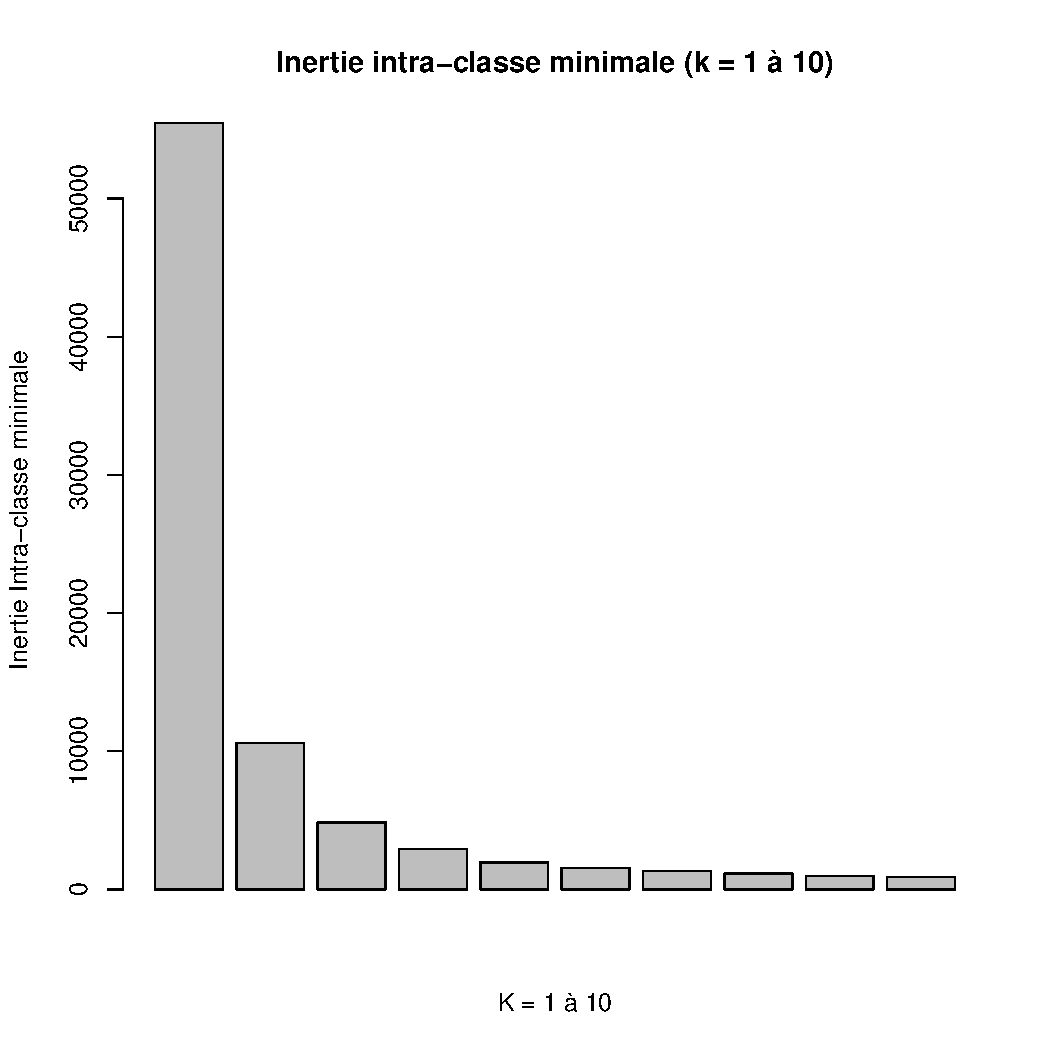
\includegraphics[width=\textwidth]{../plots/E3Q3_inertieIC.pdf}
    \caption{Evolution de la valeur de l'inertie intra-classe minimale pour la classification du dataset Iris via la méthode k-means, avec des valeurs de K allant de 1 à 10 classes}
\end{center}
\end{figure}
\paragraph{Interprétation}
En appliquant la méthode du coude à la représentation ainsi obtenue de l'évolution de l'inertie intra-classe minimale pour la classification des Iris, nous visualisons le fait que le partitionnement des Iris en K = 2 puis K = 3 classes apporte une quantité non négligeable d'information. A partir de cette dernière valeur de K, le partitionnement apporte une quantité beaucoup plus restreinte, voire négligeable d'information. Nous en déduisons que la valeur optimale du nombre de classes pour le partitionnement du dataset Iris est K = 3.
\subsection{Q4 - Comparaison des résultats de la partition obtenue par les centres mobiles avec la partition réelle des Iris en trois groupes}
\paragraph{Référence} Nous avons déjà abordé cette question au sein de notre réponse à la première question de ce troisième exercice.
\newpage
\section{Application de la méthode des centres mobiles au dataset Crabs}
\subsection{Classification des crabs en K = 2 classes}
\paragraph{Introduction}
Nous souhaitons maintenant appliquer la méthode des centres mobiles au dataset \verb+crabs2+. De la même manière, nous allons tenter de classifier les crabes en deux, puis en quatre partition. Sachant que notre dataset comporte deux espèces de crabes, et que chacune de ces espèces contient elle même 50 individus mâles et 50 individus femelles, il va être intéressant de voir si le facteur différence d'espèce implique des dissimilarités plus grandes que le facteur différence de sexe, ou l'inverse.
\paragraph{Stabilité du résultat}
Nous souhaitons dans le même temps étudier la stabilité du résultat, nous répéterons donc un grand nombre de fois l'opération de classification afin de voir si nous obtenons la même classification à chaque fois.
\paragraph{Classification}
Nous répétons donc un grand nombre de fois l'opération de classification via la méthode des k-means, afin d'observer l'évolution potentielle des résultats de son application.
\begin{figure}[ht!]
\begin{center}
    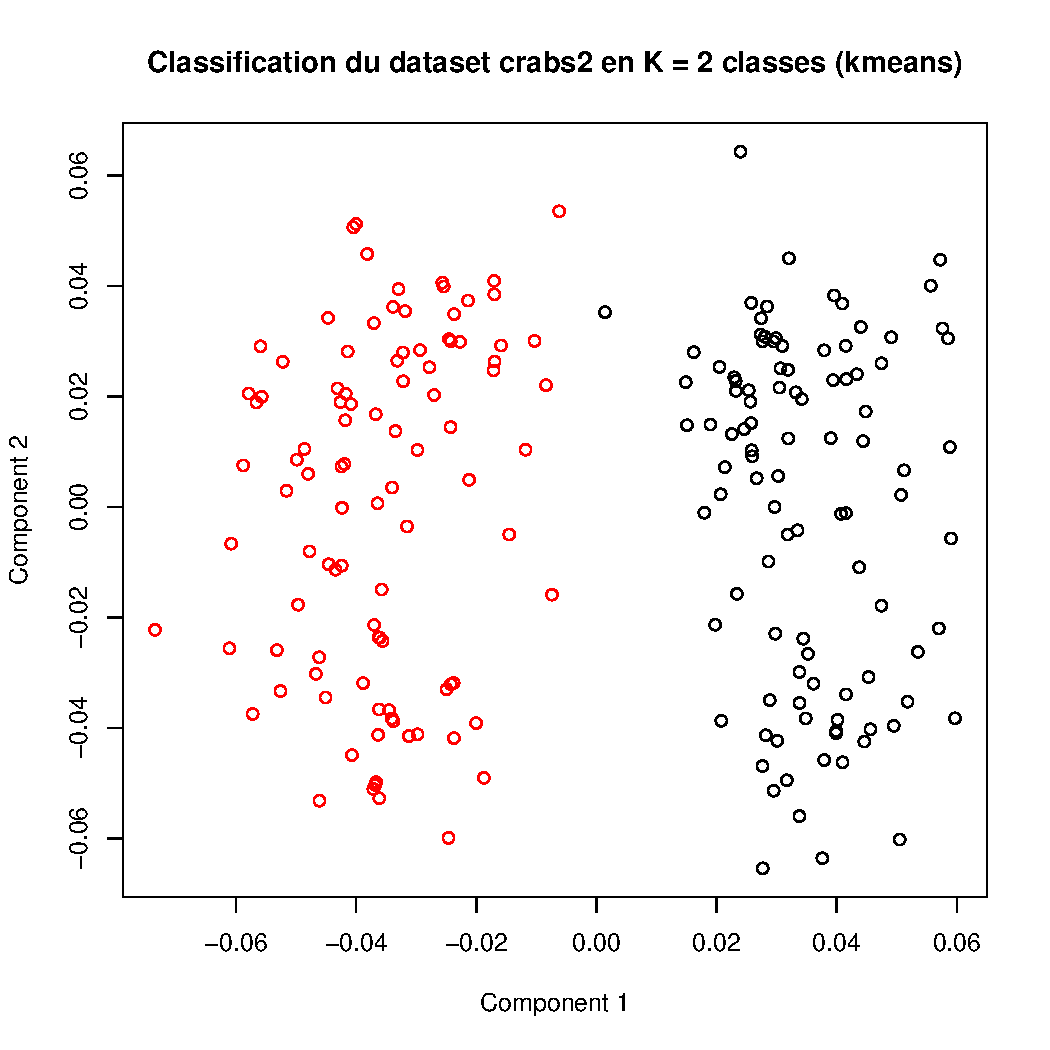
\includegraphics[width=\textwidth]{../plots/E3Q5_1.pdf}
    \caption{Classification du dataset crabs2 via la méthode des k-means en K = 2 classes (vue ACP)}
\end{center}
\end{figure}
\newpage
\paragraph{Interprétation}
Contrairement à ce que nous avons pu obtenir au cours de l'étude des Iris, cette fois ci la répétition de l'application de la méthode des k-means aux crabs n'a donné qu'un seul et unique résultat représenté ci-dessus.
\begin{figure}[ht!]
\begin{center}
    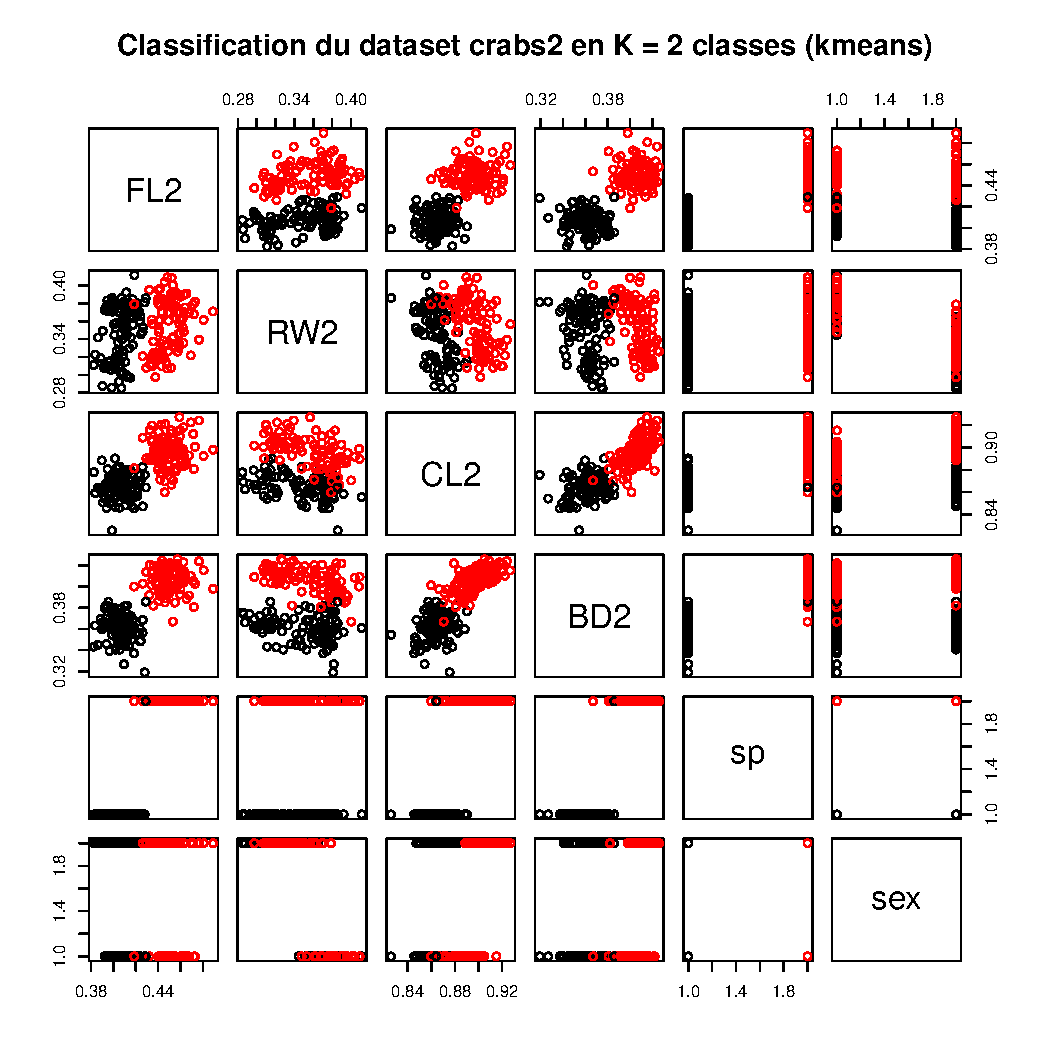
\includegraphics[width=\textwidth]{../plots/E3Q5_2.pdf}
    \caption{Classification du dataset crabs2 via la méthode des k-means en K = 2 classes (vue Pairplot)}
\end{center}
\end{figure}
\newpage
\paragraph{Interprétation}
La réprésentation en pairplot nous montre que cette classification correspond à une différenciation en fonction de l'espèce. Nous supposons donc que des individus d'espèces différentes sont fortement plus dissimilaires que des individus d'une même espèces mais de sexe différent.
\newpage
\subsection{Classification des crabs en K = 4 classes}
\paragraph{Classification}
Dans un second temps, effectuons la classification des crabes en K = 4 classes, via la méthode des k-means.
\begin{figure}[ht!]
\begin{center}
    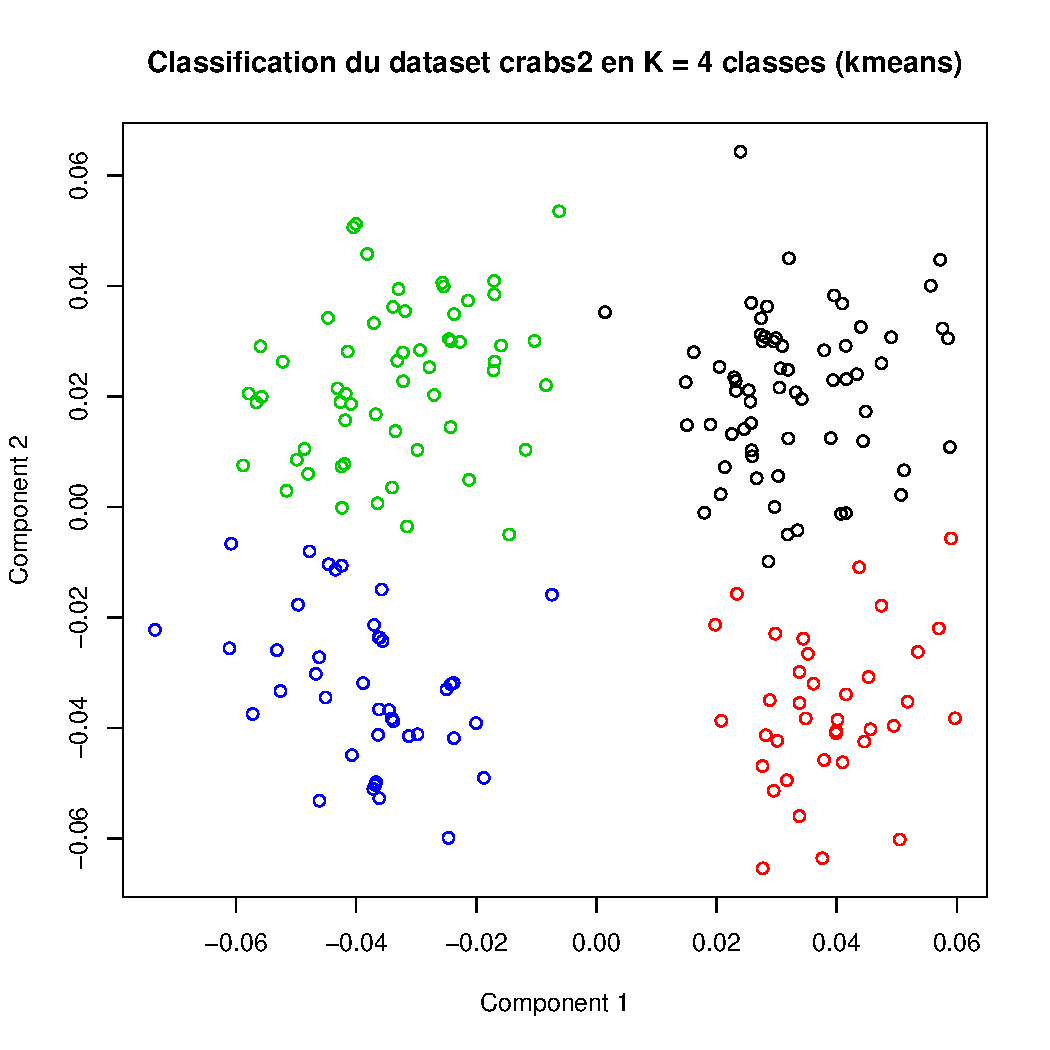
\includegraphics[width=\textwidth]{../plots/E3Q6_2.pdf}
    \caption{Classification du dataset crabs2 via la méthode des k-means en K = 4 classes (vue ACP)}
\end{center}
\end{figure}
\newpage
\begin{figure}[ht!]
\begin{center}
    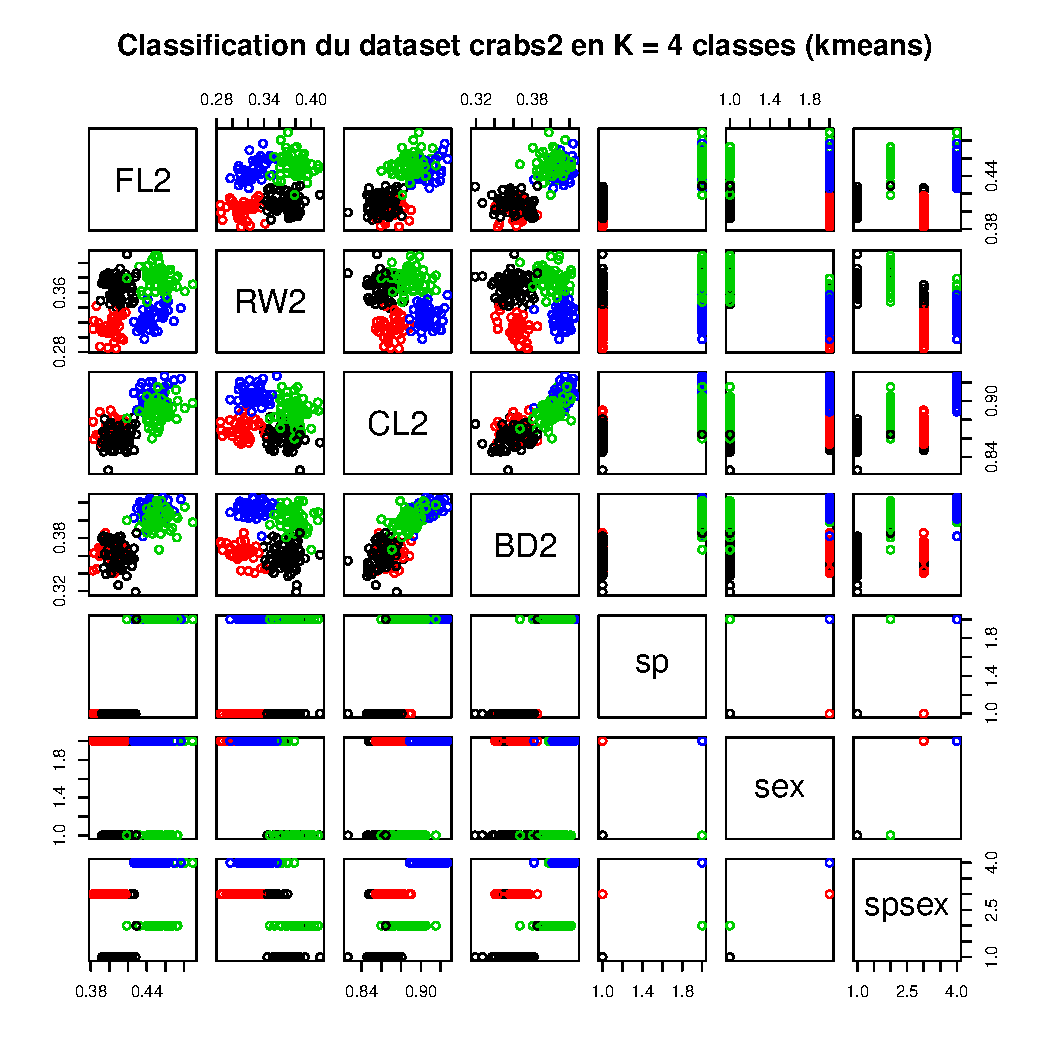
\includegraphics[width=\textwidth]{../plots/E3Q6_1.pdf}
    \caption{Classification du dataset crabs2 via la méthode des k-means en K = 4 classes (vue Pairplot)}
\end{center}
\newpage
\end{figure}
\paragraph{Interprétation}
La classification des crabs en K = 4 classes via la méthode des k-means colle globalement bien au partitionnement réel prenant en compte le sexe et l'espèce des crabs. Nous remarquons tout de même un nombre assez important d'individus, dont les caractéristiques sont assez éloignés des caractéristiques moyennes de leur classes, classés dans la mauvaise partition. Encore une fois, nous pouvons en conclure que la méthode des k-means n'assure pas une classification infaillible. Nous pouvons émettre l'hypothèse que la prise en compte d'un plus grand nombre de caractéristiques significatives nous permettrait d'affiner la précision de notre tableau de dissimilarités, et ainsi obtenir de meilleurs résultats au cours de l'application de la méthode des k-means.
\newpage
\section{Application de la méthode des centres mobiles au dataset Mutations}
\paragraph{Introduction}
Pour compléter ce TP, nous souhaitons appliquer la méthode des centres mobiles pour obtenir une classification du dataset Mutations.
\paragraph{Classification en K = 3 classes}
Nous partitionnons donc notre dataset en K = 3 classes, et représentons la classification dans le premier plan factoriel de l'AFTD. Nous étudions dans le même temps la stabilité du résultat en effectuant plusieurs tests de classification et vérifiant que nous obtenons toujours la même classification.
\begin{figure}[ht!]
\begin{center}
    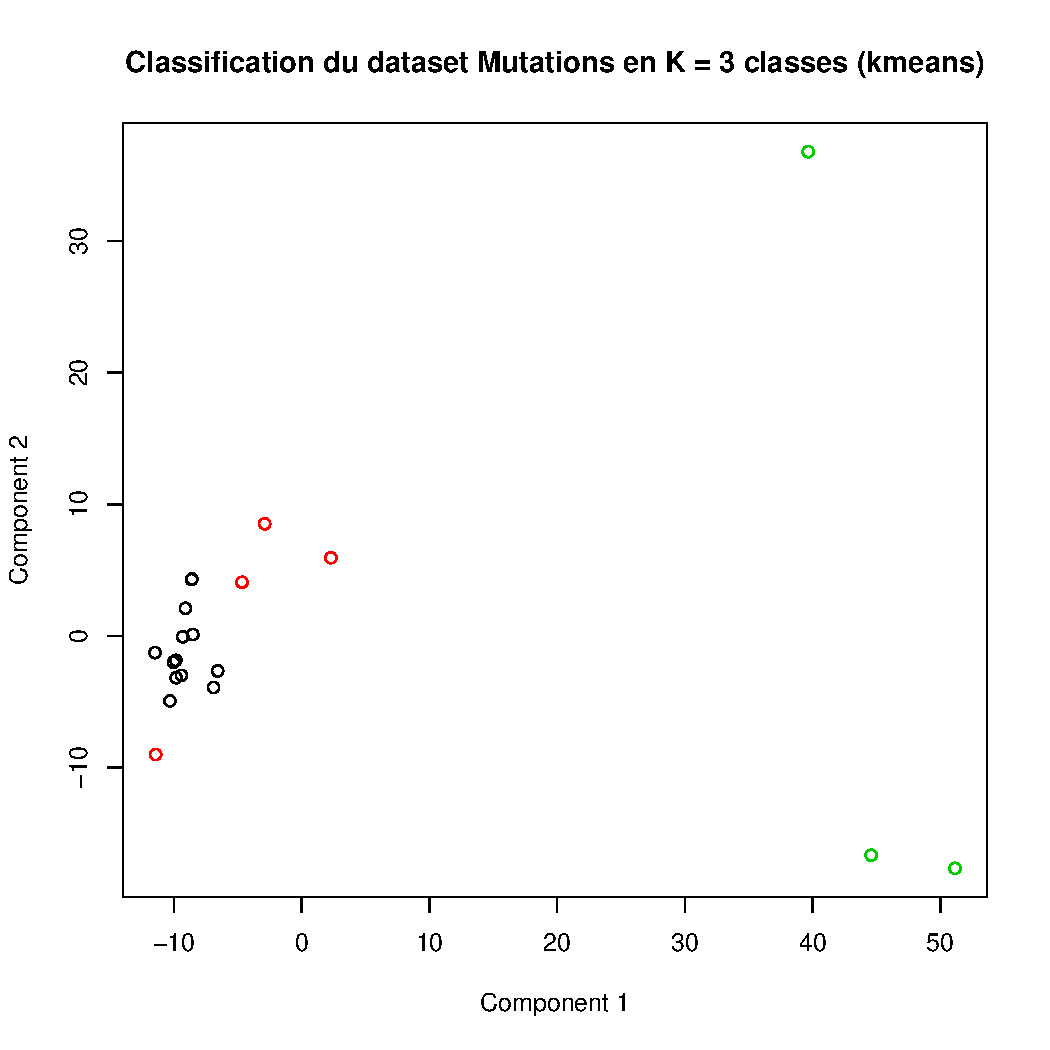
\includegraphics[width=\textwidth]{../plots/E3Q7_1.pdf}
    \caption{Classification du dataset Mutations via la méthode des k-means en K = 3 classes (vue AFTD)}
\end{center}
\end{figure}
\paragraph{Interprétation}
La classification en K = 3 classes du jeu de données Mutations met en exergue trois classes. Notons ici que le premier plan factoriel représente bien la proximité des individus de la classe noire, cependant cette représentation ne nous aurait pas permis de deviner la configuration du partitionnement des deux autres classes (nous aurions plutot eu tendance, à l'intuition, à placer les individus en rouge dans la même partition que les individus en noir, et aurions scindé les individus en deux groupes : le groupe de 2 individus, et l'individu seul).
\paragraph{Etude de la stabilité}
En répétant l'opération un grand nombre de fois, nous obtenons toujours la même classification. Notre résultat est donc relativement stable, la dissimilarité entre individus de classes différentes est avérée.
\chapter{Conclusion}
\paragraph{TP2 - Réalisations}
Ce second TP de l'UV Analyse de données et data mining (SY09) a été l'occasion pour nous de continuer notre apprentissage de la fouille de données, en appliquant notamment les méthodes de classification automatique non supervisée à trois jeux de données standards de R. Nous avons dans un premier temps consolidé nos connaissances en visualisation de données, notamment par la réalisation de deux Analyses en Composantes Principales (ACP) et une Analyse Factorielle d'un Tableau de Dissimilarités (AFTD). Nous avons ensuite su partitionner des ensembles d'invidus en classes, en appliquant trois méthodes de classification automatique que sont la classification hiérarchique ascendante, la classification hiérarchique descendante et la méthode des centres mobiles (k-means). Pour finir, nous avons étudié la stabilité de nos classifications ainsi que la manière de choisir un nombre optimal de classes de partitionement.
\paragraph{TP2 - Conclusion}
Ce TP a donc été une excellente mise en pratique de nos connaissances théoriques sur la classification automatique non supervisée. Nous avons pu constater l'utilité de cette dernière lorsqu'il s'agit de dégager des caractéristiques communes au sein d'un ensemble d'individus et noté l'importance de trouver un bon compromis entre généralisation de l'information, et homogénéité des partitions résultantes.
\end{document}
